\documentclass[12pt,dvipdfmx]{article}
\usepackage{amsmath,amssymb}
\usepackage[a3paper,landscape,top=25mm,bottom=25mm,left=25mm,right=25mm]{geometry}
%\usepackage[dvipdfmx]{graphicx}
\usepackage{amsthm}
%\usepackage{bm}
\usepackage{tikz}
\usetikzlibrary{arrows}
\usetikzlibrary{arrows.meta,chains,matrix,decorations.pathreplacing,bending}
%\usepackage{framed}
%\usepackage{ascmac}
%\usepackage{cancel}
\usepackage{mathrsfs}
\usepackage[noadjust]{cite}
\usepackage{type1cm}
\usepackage{mathtools}\mathtoolsset{showonlyrefs=true}
\usetikzlibrary{intersections,math,patterns}
%\usepackage[useregional]{datetime2}
\definecolor{blue1}{rgb}{0.0156863, 0.0235294, 0.0705882}
\definecolor{blue2}{rgb}{0.0196078, 0.0431373, 0.0980392}
\definecolor{blue3}{rgb}{0.027451, 0.0705882, 0.14902}
\definecolor{blue4}{rgb}{0.0313725, 0.0705882, 0.145098}
\definecolor{blue5}{rgb}{0.0431373, 0.0901961, 0.180392}
\definecolor{blue6}{rgb}{0.0431373, 0.0901961, 0.184314}
\definecolor{blue7}{rgb}{0.0509804, 0.113725, 0.211765}
\definecolor{blue8}{rgb}{0.0666667, 0.145098, 0.25098}
\definecolor{blue9}{rgb}{0.0862745, 0.176471, 0.286275}
\definecolor{blue10}{rgb}{0.0980392, 0.2, 0.317647}
\definecolor{blue11}{rgb}{0.121569, 0.243137, 0.356863}
\definecolor{blue12}{rgb}{0.137255, 0.278431, 0.384314}
\definecolor{blue13}{rgb}{0.160784, 0.333333, 0.447059}
% \definecolor{black14}{rgb}{47,91,131}
\definecolor{blue14}{rgb}{0.184314, 0.356863, 0.513725}
\definecolor{coolblack}{rgb}{0.0, 0.18, 0.39}
\definecolor{harvestgold}{rgb}{0.85, 0.57, 0.0}
% \definecolor{ivory}{rgb}{1.0, 1.0, 0.94}
\definecolor{ivory}{rgb}{0.9, 0.9, 0.84}
\definecolor{lapislazuli}{rgb}{0.15, 0.38, 0.61}
\definecolor{darkjunglegreen}{rgb}{0.15, 0.14, 0.13}
\definecolor{deepjunglegreen}{rgb}{0.0, 0.29, 0.29}
\definecolor{mediumjunglegreen}{rgb}{0.11, 0.21, 0.18}
\definecolor{indianred}{rgb}{0.8, 0.36, 0.36}





%text font
%\usepackage[math]{anttor}
\let\Bbbk\relax\usepackage{newtxtext}
\usepackage[lite,subscriptcorrection,slantedGreek,nofontinfo]{mtpro2}
\usepackage{bbold}
%\usepackage{newtxmath}
%\usepackage{mbboard}
%\usepackage[condensed,math]{kurier}

\setlength{\textwidth}{\paperwidth}     % 紙面横幅を本文領域にする(RIGHT=-LEFT)
\setlength{\oddsidemargin}{-0.4truemm}  % 左の余白を25mm(=1inch-0.4mm)に
\setlength{\evensidemargin}{-0.4truemm} % 
\addtolength{\textwidth}{-50truemm}     % 右の余白も25mm(RIGHT=-LEFT)

\title{New Template}
\author{19lc001a Kento Fujita}
\pagestyle{myheadings}

\newtheorem{theorem}{Theorem}[section]
\newtheorem{conjecture}{Conjecture}[section]
\newtheorem{lemma}{Lemma}[section]
\newtheorem{corollary}{Corollary}[section]
\newtheorem{proposition}{Proposition}[section]

\theoremstyle{definition}
\newtheorem{definition}{Definition}[section]

\theoremstyle{remark}
\newtheorem*{remark}{Remark}

\numberwithin{equation}{section}



\DeclareMathOperator{\dep}{dep}
\DeclareMathOperator{\wt}{wt}
\DeclareMathOperator{\height}{ht}
\DeclareMathOperator{\Li}{Li}
\newcommand{\myLi}{\mathscr{L}}
\newcommand{\hgf}[5]{{\mathchoice%
{{}_{#1}F_{#2}\!\left(\genfrac{}{}{0pt}{}{#3}{#4}\,;\,#5\right)}% display mode
{{}_{#1}F_{#2}(#3;#4;#5)}% text mode
{}{}}}
\def\us#1_#2{\underset{#2}{#1}}
\def\os#1^#2{\overset{#2}{#1}}
\DeclareFontFamily{U}{wncy}{}
\DeclareFontShape{U}{wncy}{m}{n}{<->wncyr10}{}
\DeclareSymbolFont{mcy}{U}{wncy}{m}{n}
\DeclareMathSymbol{\Sh}{\mathord}{mcy}{`X}
\DeclareMathSymbol{\sh}{\mathord}{mcy}{`x}


\makeatletter
\pgfkeys{%
  /pgf/decoration/.cd,
  start color/.store in =\startcolor,
  end color/.store in   =\endcolor,
  start width/.store in =\startwidth,% not used
  end width/.store in   =\endwidth,% not used
  start color=black!5,
  end color=black,
}
\pgfdeclaredecoration{width and color change}{initial}{
 \state{initial}[width=0pt, next state=line, persistent precomputation={%
   \pgfmathdivide{.5pt}{\pgfdecoratedpathlength}% not sure why .5pt works better than .75pt
   \let\increment=\pgfmathresult
   \def\x{0}%
 }]{}
 \state{line}[width=.5pt, persistent postcomputation={%
     \pgfmathadd@{\x}{\increment}%
     \let\x=\pgfmathresult
   }]{%
   \pgfsetlinewidth{\x\maxlinewidth}%
   \pgfsetarrows{-}%
   \pgfpathmoveto{\pgfpointorigin}%
   \pgfpathlineto{\pgfqpoint{.75pt}{0pt}}%
   \pgfmathmultiply{100}{\x}%
   \let\y=\pgfmathresult
   \pgfsetstrokecolor{\endcolor!\y!\startcolor}%
   \pgfusepath{stroke}%
 }
 \state{final}{%
   \pgfsetlinewidth{\pgflinewidth}%
   \pgfpathmoveto{\pgfpointorigin}%
   \color{\endcolor!\x!\startcolor}%
   \pgfusepath{stroke}%
 }
}
\makeatother

\newlength{\maxlinewidth}
\maxlinewidth=2pt


\usepackage[useregional]{datetime2}
\begin{document}
% \hfill\texttt{\jobname.tex}\qquad\DTMnow
\section{Memo}


% \begin{center}
%     \begin{tikzpicture}
%         \coordinate (O) at (0,0);
%         \coordinate (A) at (0,-2);
%         \coordinate (B) at (1.29377,-0.759051);
%         \coordinate (C) at (1.53209,-1.28558);

%         \draw [fill=black] (O) circle (2);
%         \draw [fill=white] (-0.1,-0.1) circle (1.88);
%         \draw (0,0.3) node [anchor=north]{$\mathcal{A}$ world};
    
%         \draw [fill=black] (A) to [out=10,in=-110] (B) to [out=-90,in=200] (C) to [out=-135,in=0] (A); 

%         \foreach \angle / \label in 
%         {0/$\cdot$, 15/$\cdot$, 30/$\cdot$, 45/$\cdot$, 60/$\cdot$,75/$\cdot$, 90/$\cdot$, 
%         105/$\cdot$, 120/$\cdot$, 135/$\cdot$, 150/$\cdot$, 165/$\cdot$,
%         180/$\cdot$, 190/\rotatebox{-80}{$>$}, 205/$2$, 220/\rotatebox{-50}{$>$}, 235/$1$, 
%         250/\rotatebox{-20}{$>$}, 270/$0\equiv p$, 290/\rotatebox{20}{$>$}, 305/$\ \ p-1$, 
%         320/\rotatebox{50}{$>$}, 335/$\ \ p-2$, 350/\rotatebox{80}{$>$}} 
%         { 
%       %    \draw (\angle:1.8cm) -- (\angle:2cm); 
%          \node at (\angle:2.5cm) {\textsf{\label}}; 
%         } 

%     \end{tikzpicture}
% \end{center}


% \begin{center}
%     \begin{tikzpicture}
%         \coordinate (O) at (0,0);
%         \coordinate (A) at (0,-2);
%         \coordinate (B) at (1.29377,-0.759051);
%         \coordinate (C) at (1.53209,-1.28558);

%         \draw [fill=black] (O) circle (2);
%         \draw [fill=white] (-0.1,-0.1) circle (1.88);
%         \draw (0,0.3) node [anchor=north]{Kontsevich's world};
    
%         \draw [fill=black] (A) to [out=10,in=-110] (B) to [out=-90,in=200] (C) to [out=-135,in=0] (A); 

%         \foreach \angle / \label in 
%         {0/$\cdot$, 15/$\cdot$, 30/$\cdot$, 45/$\cdot$, 60/\rotatebox{-30}{$<$}, 90/$``\infty=-\infty"$, 
%         120/\rotatebox{30}{$<$}, 135/$\cdot$, 150/$\cdot$, 165/$\cdot$,
%         180/$\cdot$, 190/\rotatebox{-80}{$>$}, 205/$2$, 220/\rotatebox{-50}{$>$}, 235/$1$, 
%         250/\rotatebox{-20}{$>$}, 270/$0$, 290/\rotatebox{20}{$>$}, 305/$\ \ -1$, 
%         320/\rotatebox{50}{$>$}, 335/$\ \ -2$, 350/\rotatebox{80}{$>$}} 
%         { 
%       %    \draw (\angle:1.8cm) -- (\angle:2cm); 
%          \node at (\angle:2.5cm) {\textsf{\label}}; 
%         } 

%     \end{tikzpicture}
% \end{center}

% \begin{center}
  %%%%%緑のやつ
  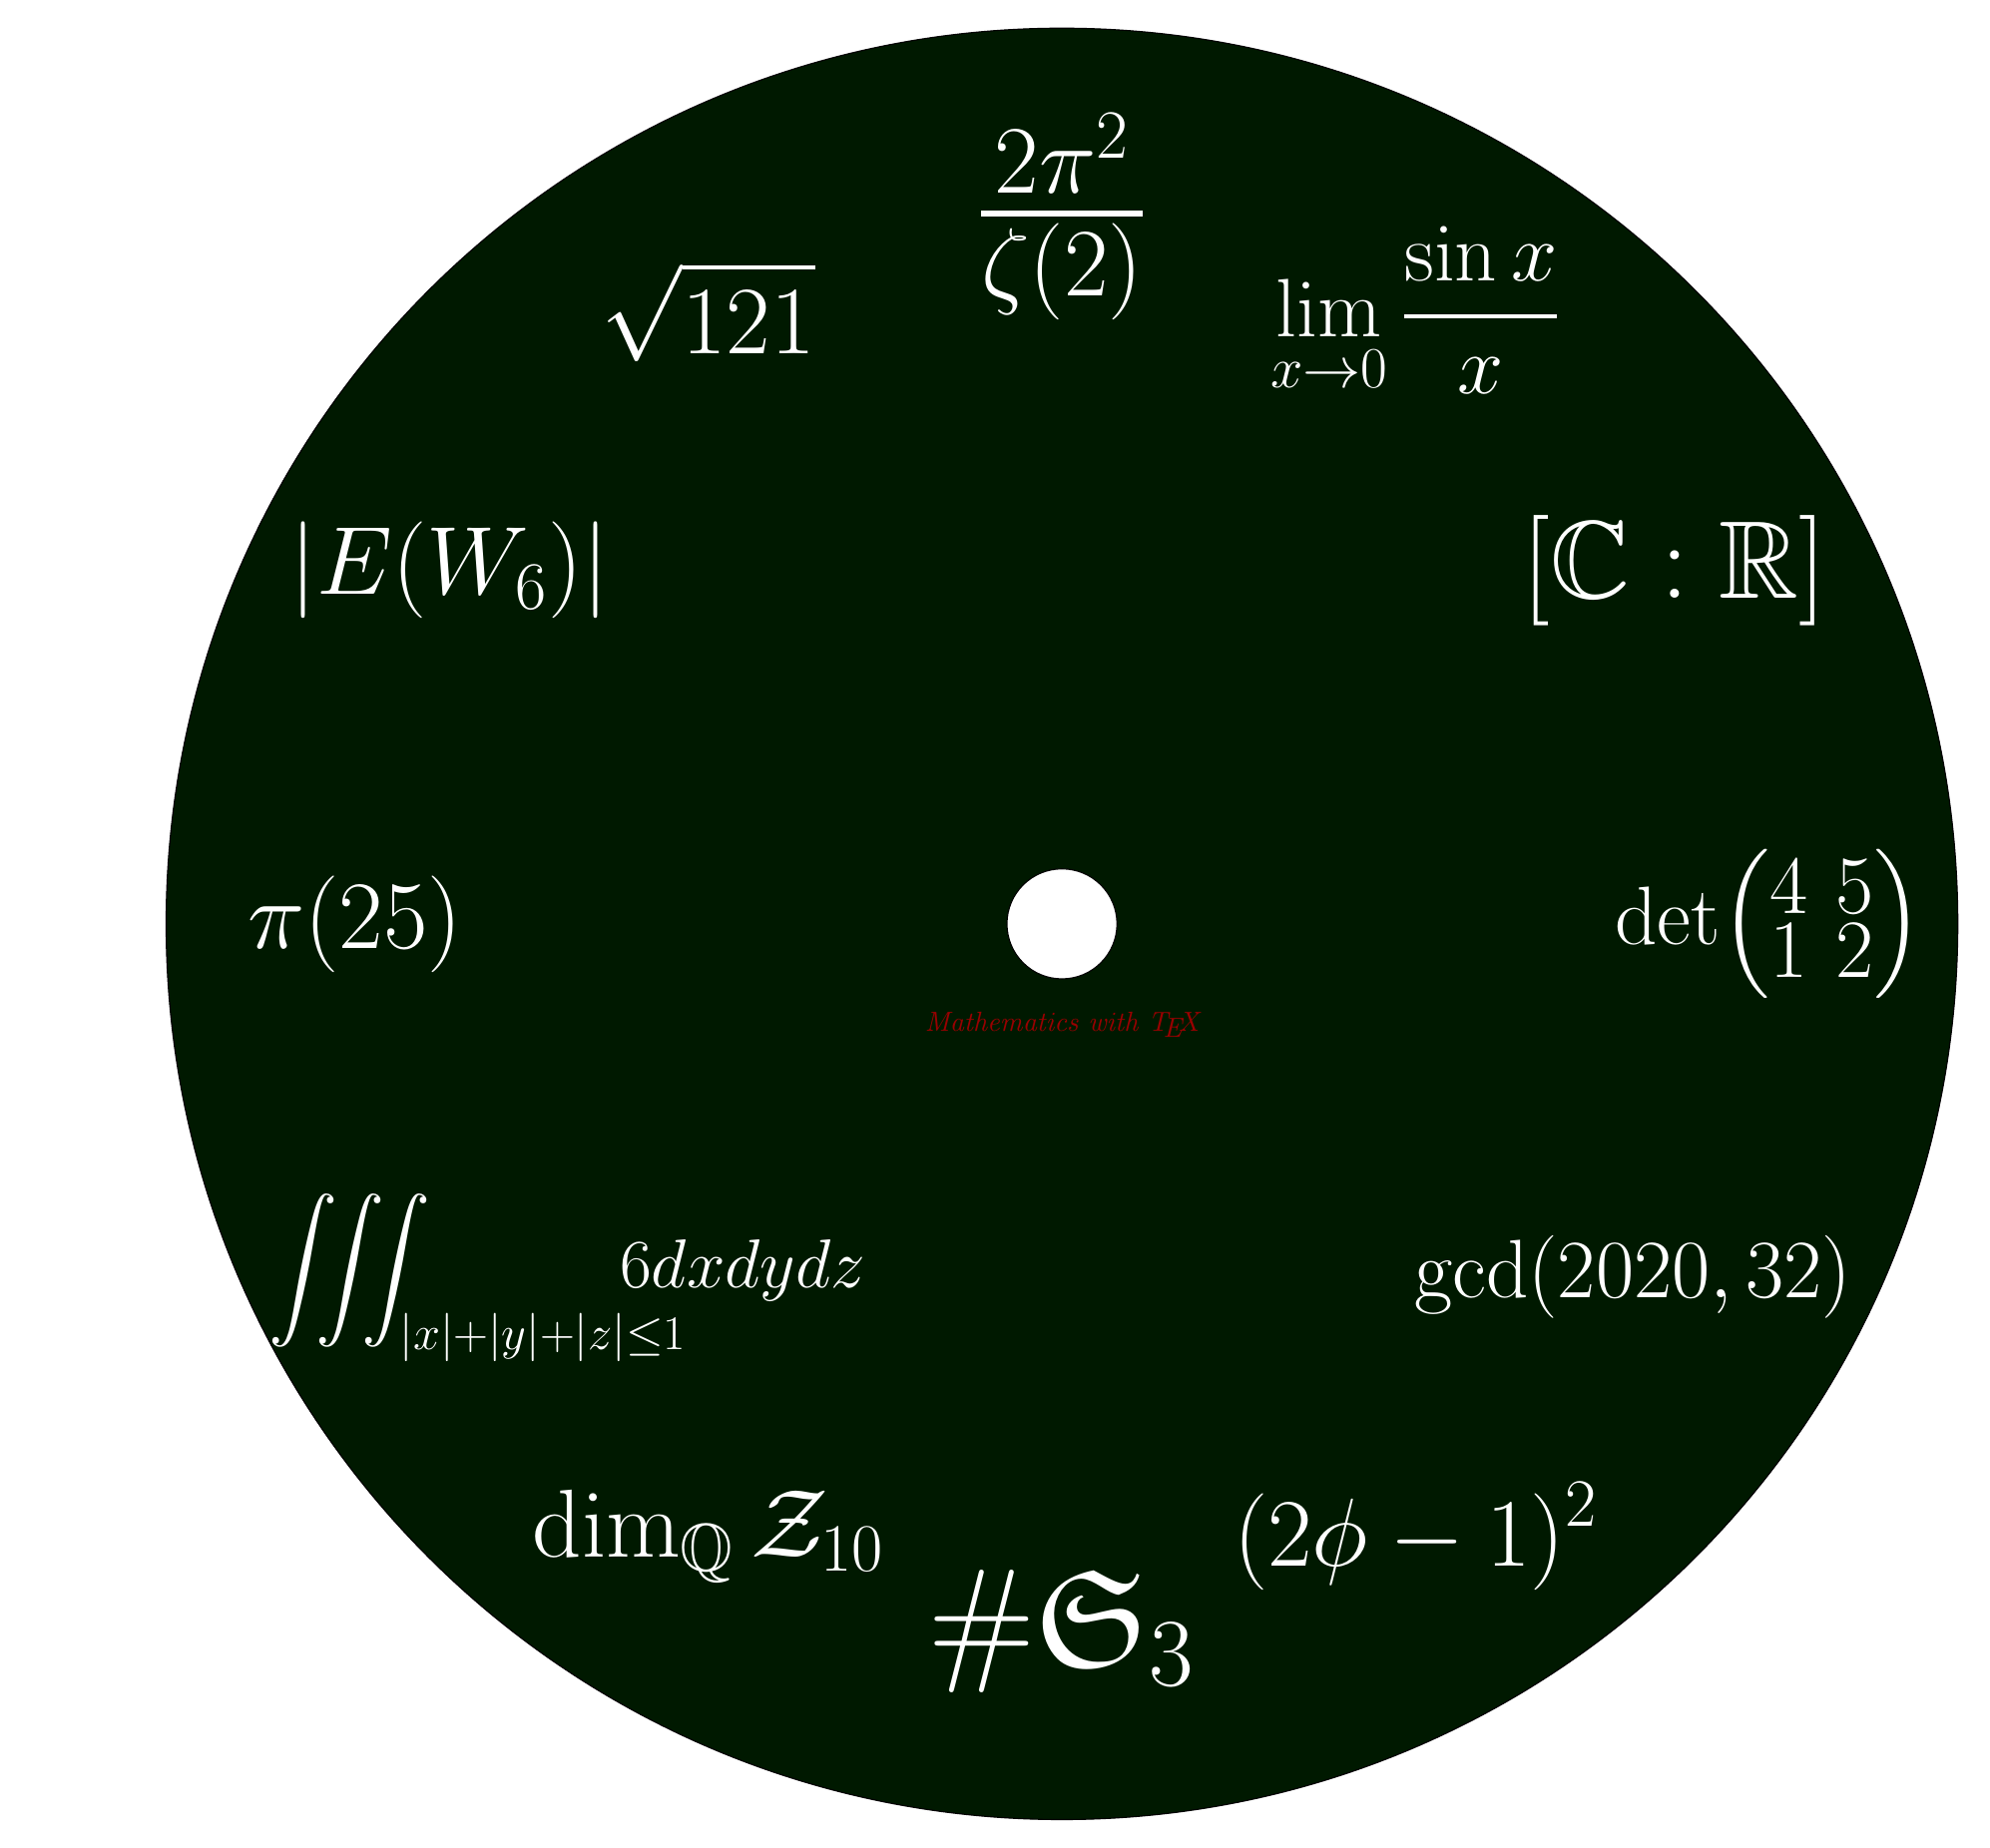
\begin{tikzpicture}
      \coordinate (O) at (0,0);
      \coordinate (A) at (0,-2);
      \coordinate (B) at (1.29377,-0.759051);
      \coordinate (C) at (1.53209,-1.28558);

      \draw [fill=black!90!green](O) circle (11.4cm);
      \draw [fill=white] (O) circle (7mm);
      \draw (0,-1) node [anchor=north]{\textit{\textcolor{red!60!black}{Mathematics with \TeX}}};
      % \draw [fill=white] (-0.1,-0.1) circle (1.88);
      % \draw (0,0.3) node [anchor=north]{Kontsevich's world};
  
      % \draw [fill=black] (A) to [out=10,in=-110] (B) to [out=-90,in=200] (C) to [out=-135,in=0] (A); 

      \foreach \angle / \label in 
      {
        0/\fontsize{30}{10}{\textcolor{white}{$\det\!\begin{pmatrix}4&5\\1 &2\end{pmatrix}$}},
        30/\fontsize{40}{10}{\textcolor{white}{$\displaystyle[\mathbb{C}:\mathbb{R}]$}},
        60/\fontsize{30}{10}{\textcolor{white}{$\displaystyle\lim_{x\rightarrow 0}\frac{\sin x}{x}$}},
        90/\fontsize{50}{10}{\textcolor{white}{$\frac{2\pi^2}{\zeta(2)}$}},
        120/\fontsize{35}{10}{\textcolor{white}{$\displaystyle\sqrt{121}$}},
        150/\fontsize{35}{10}{\textcolor{white}{$\displaystyle|E(W_6)|$}},
        180/\fontsize{35}{10}{\textcolor{white}{$\displaystyle\pi(25)$}},
        210/\fontsize{25}{10}{\textcolor{white}{$\hspace{30mm}\displaystyle\us\iiint_{|x|+|y|+|z|\leq 1}\hspace{-10mm}6dxdydz$}},
        240/\fontsize{35}{10}{\textcolor{white}{$\displaystyle\dim_\mathbb{Q}\mathcal{Z}_{10}$}},
        270/\fontsize{50}{10}{\textcolor{white}{$\#\mathfrak{S}_3$}},
        300/\fontsize{35}{10}{\textcolor{white}{$\displaystyle(2\phi -1)^2$}},
        330/\fontsize{30}{10}{\textcolor{white}{$\displaystyle\gcd(2020,32)\ \ \ \ \ \ \ \ \ $}}
      } 
      { 
      %  \draw (\angle:22cm) -- (\angle:12cm); 
       \node at (\angle:9cm) {\textsf{\label}}; 
      } 

  \end{tikzpicture}
  \newpage
  %灰色のやつ
  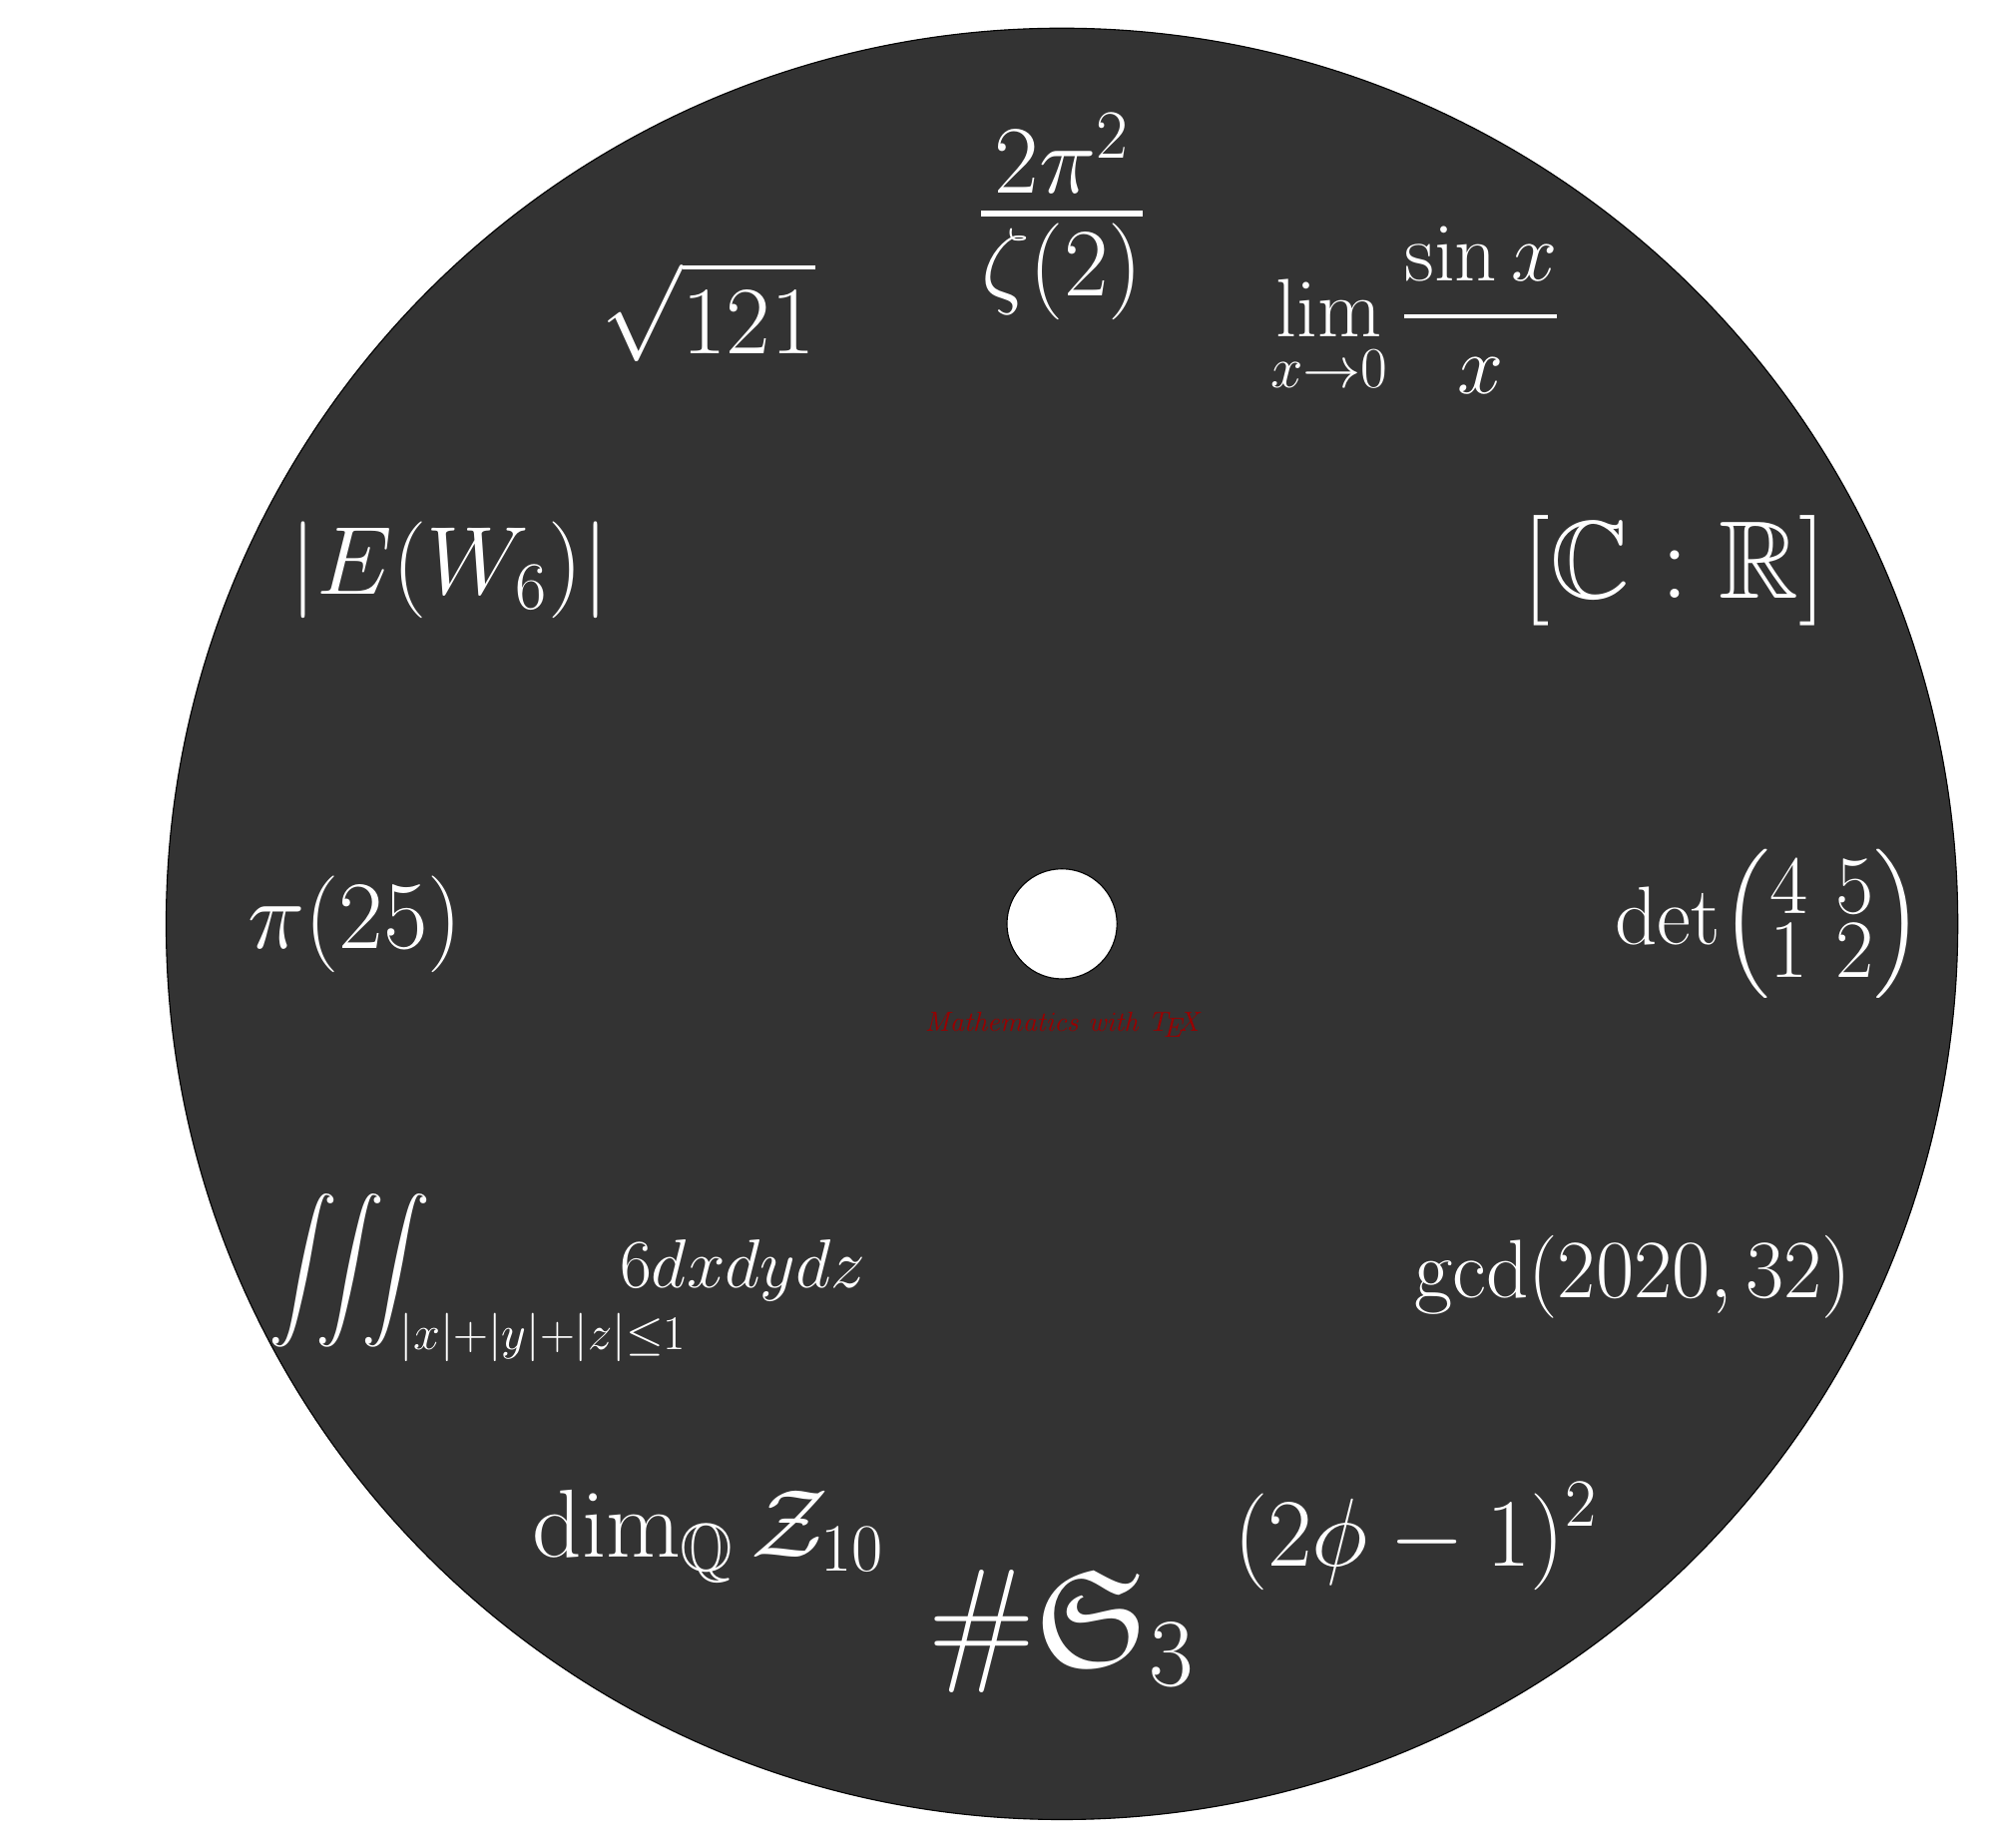
\begin{tikzpicture}
    \coordinate (O) at (0,0);
    \coordinate (A) at (0,-2);
    \coordinate (B) at (1.29377,-0.759051);
    \coordinate (C) at (1.53209,-1.28558);

    \draw [fill=black!80!white](O) circle (11.4cm);
    \draw [fill=white] (O) circle (7mm);
    \draw (0,-1) node [anchor=north]{\textit{\textcolor{red!60!black}{Mathematics with \TeX}}};
    % \draw [fill=white] (-0.1,-0.1) circle (1.88);
    % \draw (0,0.3) node [anchor=north]{Kontsevich's world};

    % \draw [fill=black] (A) to [out=10,in=-110] (B) to [out=-90,in=200] (C) to [out=-135,in=0] (A); 

    \foreach \angle / \label in 
    {
      0/\fontsize{30}{10}{\textcolor{white}{$\det\!\begin{pmatrix}4&5\\1 &2\end{pmatrix}$}},
      30/\fontsize{40}{10}{\textcolor{white}{$\displaystyle[\mathbb{C}:\mathbb{R}]$}},
      60/\fontsize{30}{10}{\textcolor{white}{$\displaystyle\lim_{x\rightarrow 0}\frac{\sin x}{x}$}},
      90/\fontsize{50}{10}{\textcolor{white}{$\frac{2\pi^2}{\zeta(2)}$}},
      120/\fontsize{35}{10}{\textcolor{white}{$\displaystyle\sqrt{121}$}},
      150/\fontsize{35}{10}{\textcolor{white}{$\displaystyle|E(W_6)|$}},
      180/\fontsize{35}{10}{\textcolor{white}{$\displaystyle\pi(25)$}},
      210/\fontsize{25}{10}{\textcolor{white}{$\hspace{30mm}\displaystyle\us\iiint_{|x|+|y|+|z|\leq 1}\hspace{-10mm}6dxdydz$}},
      240/\fontsize{35}{10}{\textcolor{white}{$\displaystyle\dim_\mathbb{Q}\mathcal{Z}_{10}$}},
      270/\fontsize{50}{10}{\textcolor{white}{$\#\mathfrak{S}_3$}},
      300/\fontsize{35}{10}{\textcolor{white}{$\displaystyle(2\phi -1)^2$}},
      330/\fontsize{30}{10}{\textcolor{white}{$\displaystyle\gcd(2020,32)\ \ \ \ \ \ \ \ \ $}}
    } 
    { 
    %  \draw (\angle:22cm) -- (\angle:12cm); 
     \node at (\angle:9cm) {\textsf{\label}}; 
    } 

\end{tikzpicture}
\newpage

%黒色のやつ
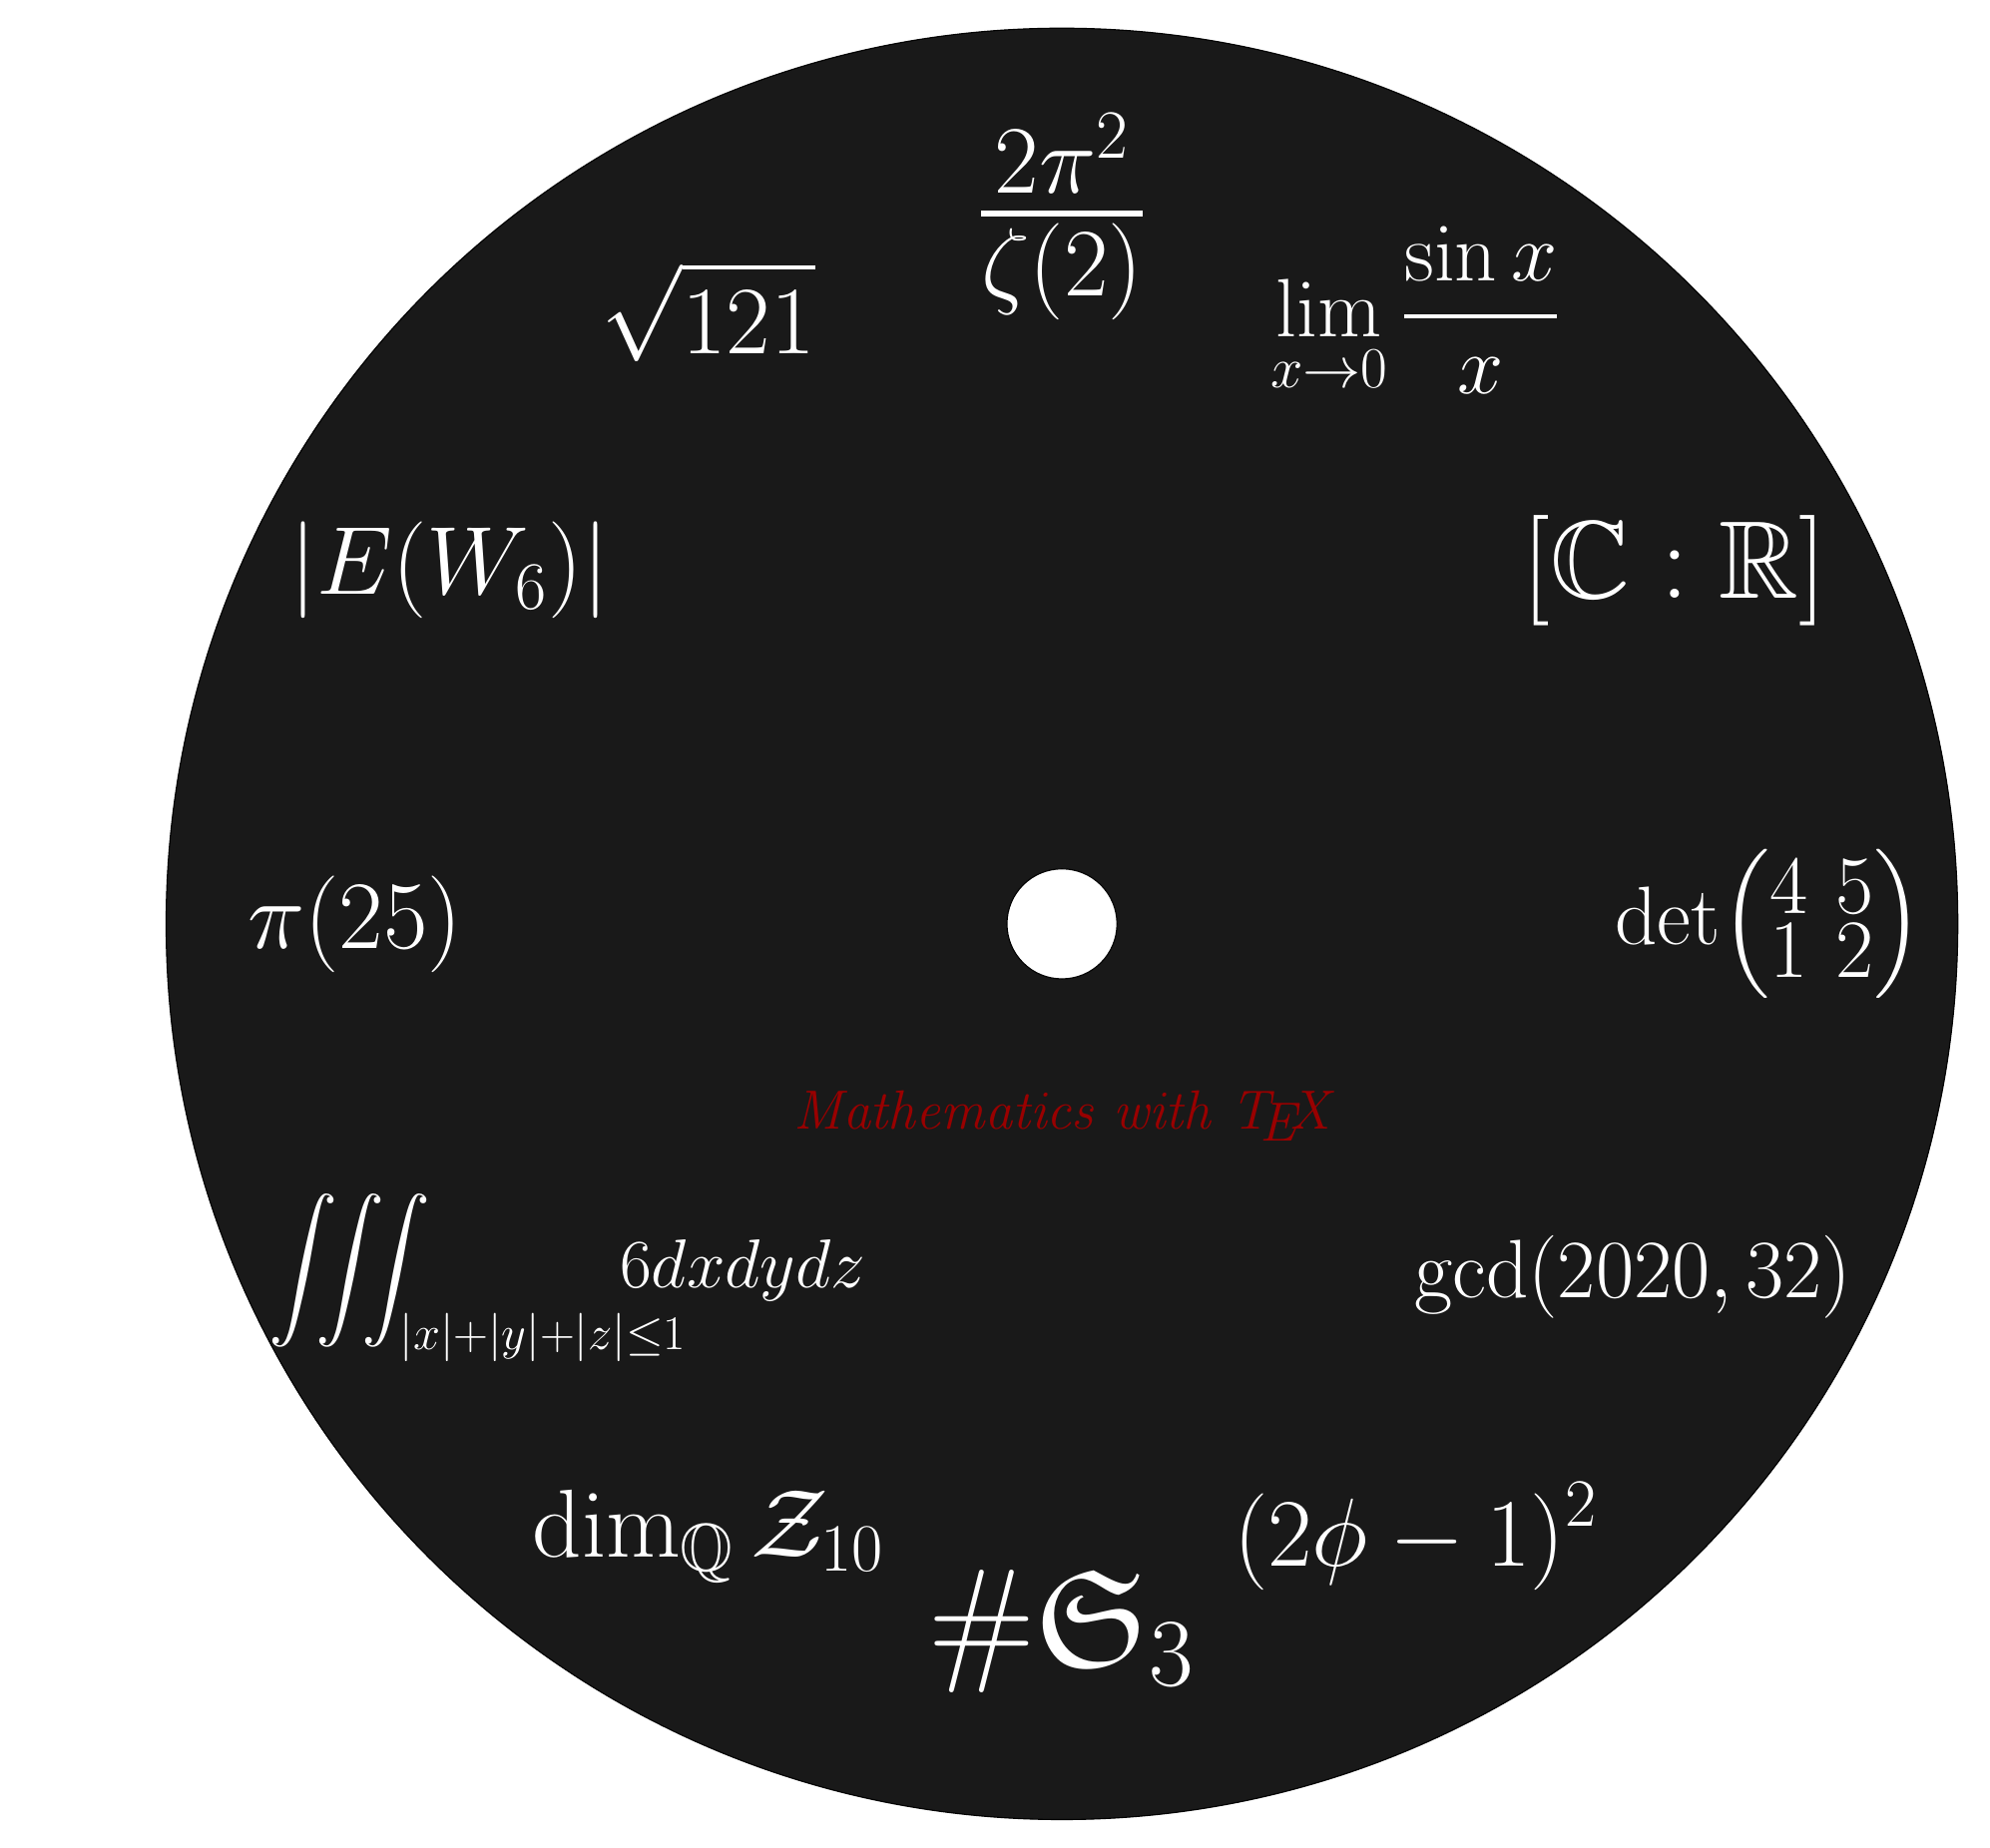
\begin{tikzpicture}
  \coordinate (O) at (0,0);
  \coordinate (A) at (0,-2);
  \coordinate (B) at (1.29377,-0.759051);
  \coordinate (C) at (1.53209,-1.28558);

  \draw [fill=black!90!white](O) circle (11.4cm);
  \draw [fill=white] (O) circle (7mm);
  \draw (0,-2) node [anchor=north]{\fontsize{20}{10}{\textit{\textcolor{red!60!black}{Mathematics with \TeX}}}};
  % \draw [fill=white] (-0.1,-0.1) circle (1.88);
  % \draw (0,0.3) node [anchor=north]{Kontsevich's world};

  % \draw [fill=black] (A) to [out=10,in=-110] (B) to [out=-90,in=200] (C) to [out=-135,in=0] (A); 

  \foreach \angle / \label in 
  {
    0/\fontsize{30}{10}{\textcolor{white}{$\det\!\begin{pmatrix}4&5\\1 &2\end{pmatrix}$}},
    30/\fontsize{40}{10}{\textcolor{white}{$\displaystyle[\mathbb{C}:\mathbb{R}]$}},
    60/\fontsize{30}{10}{\textcolor{white}{$\displaystyle\lim_{x\rightarrow 0}\frac{\sin x}{x}$}},
    90/\fontsize{50}{10}{\textcolor{white}{$\frac{2\pi^2}{\zeta(2)}$}},
    120/\fontsize{35}{10}{\textcolor{white}{$\displaystyle\sqrt{121}$}},
    150/\fontsize{35}{10}{\textcolor{white}{$\displaystyle|E(W_6)|$}},
    180/\fontsize{35}{10}{\textcolor{white}{$\displaystyle\pi(25)$}},
    210/\fontsize{25}{10}{\textcolor{white}{$\hspace{30mm}\displaystyle\us\iiint_{|x|+|y|+|z|\leq 1}\hspace{-10mm}6dxdydz$}},
    240/\fontsize{35}{10}{\textcolor{white}{$\displaystyle\dim_\mathbb{Q}\mathcal{Z}_{10}$}},
    270/\fontsize{50}{10}{\textcolor{white}{$\#\mathfrak{S}_3$}},
    300/\fontsize{35}{10}{\textcolor{white}{$\displaystyle(2\phi -1)^2$}},
    330/\fontsize{30}{10}{\textcolor{white}{$\displaystyle\gcd(2020,32)\ \ \ \ \ \ \ \ \ $}}
  } 
  { 
  %  \draw (\angle:22cm) -- (\angle:12cm); 
   \node at (\angle:9cm) {\textsf{\label}}; 
  } 

\end{tikzpicture}

%黒色のやつ
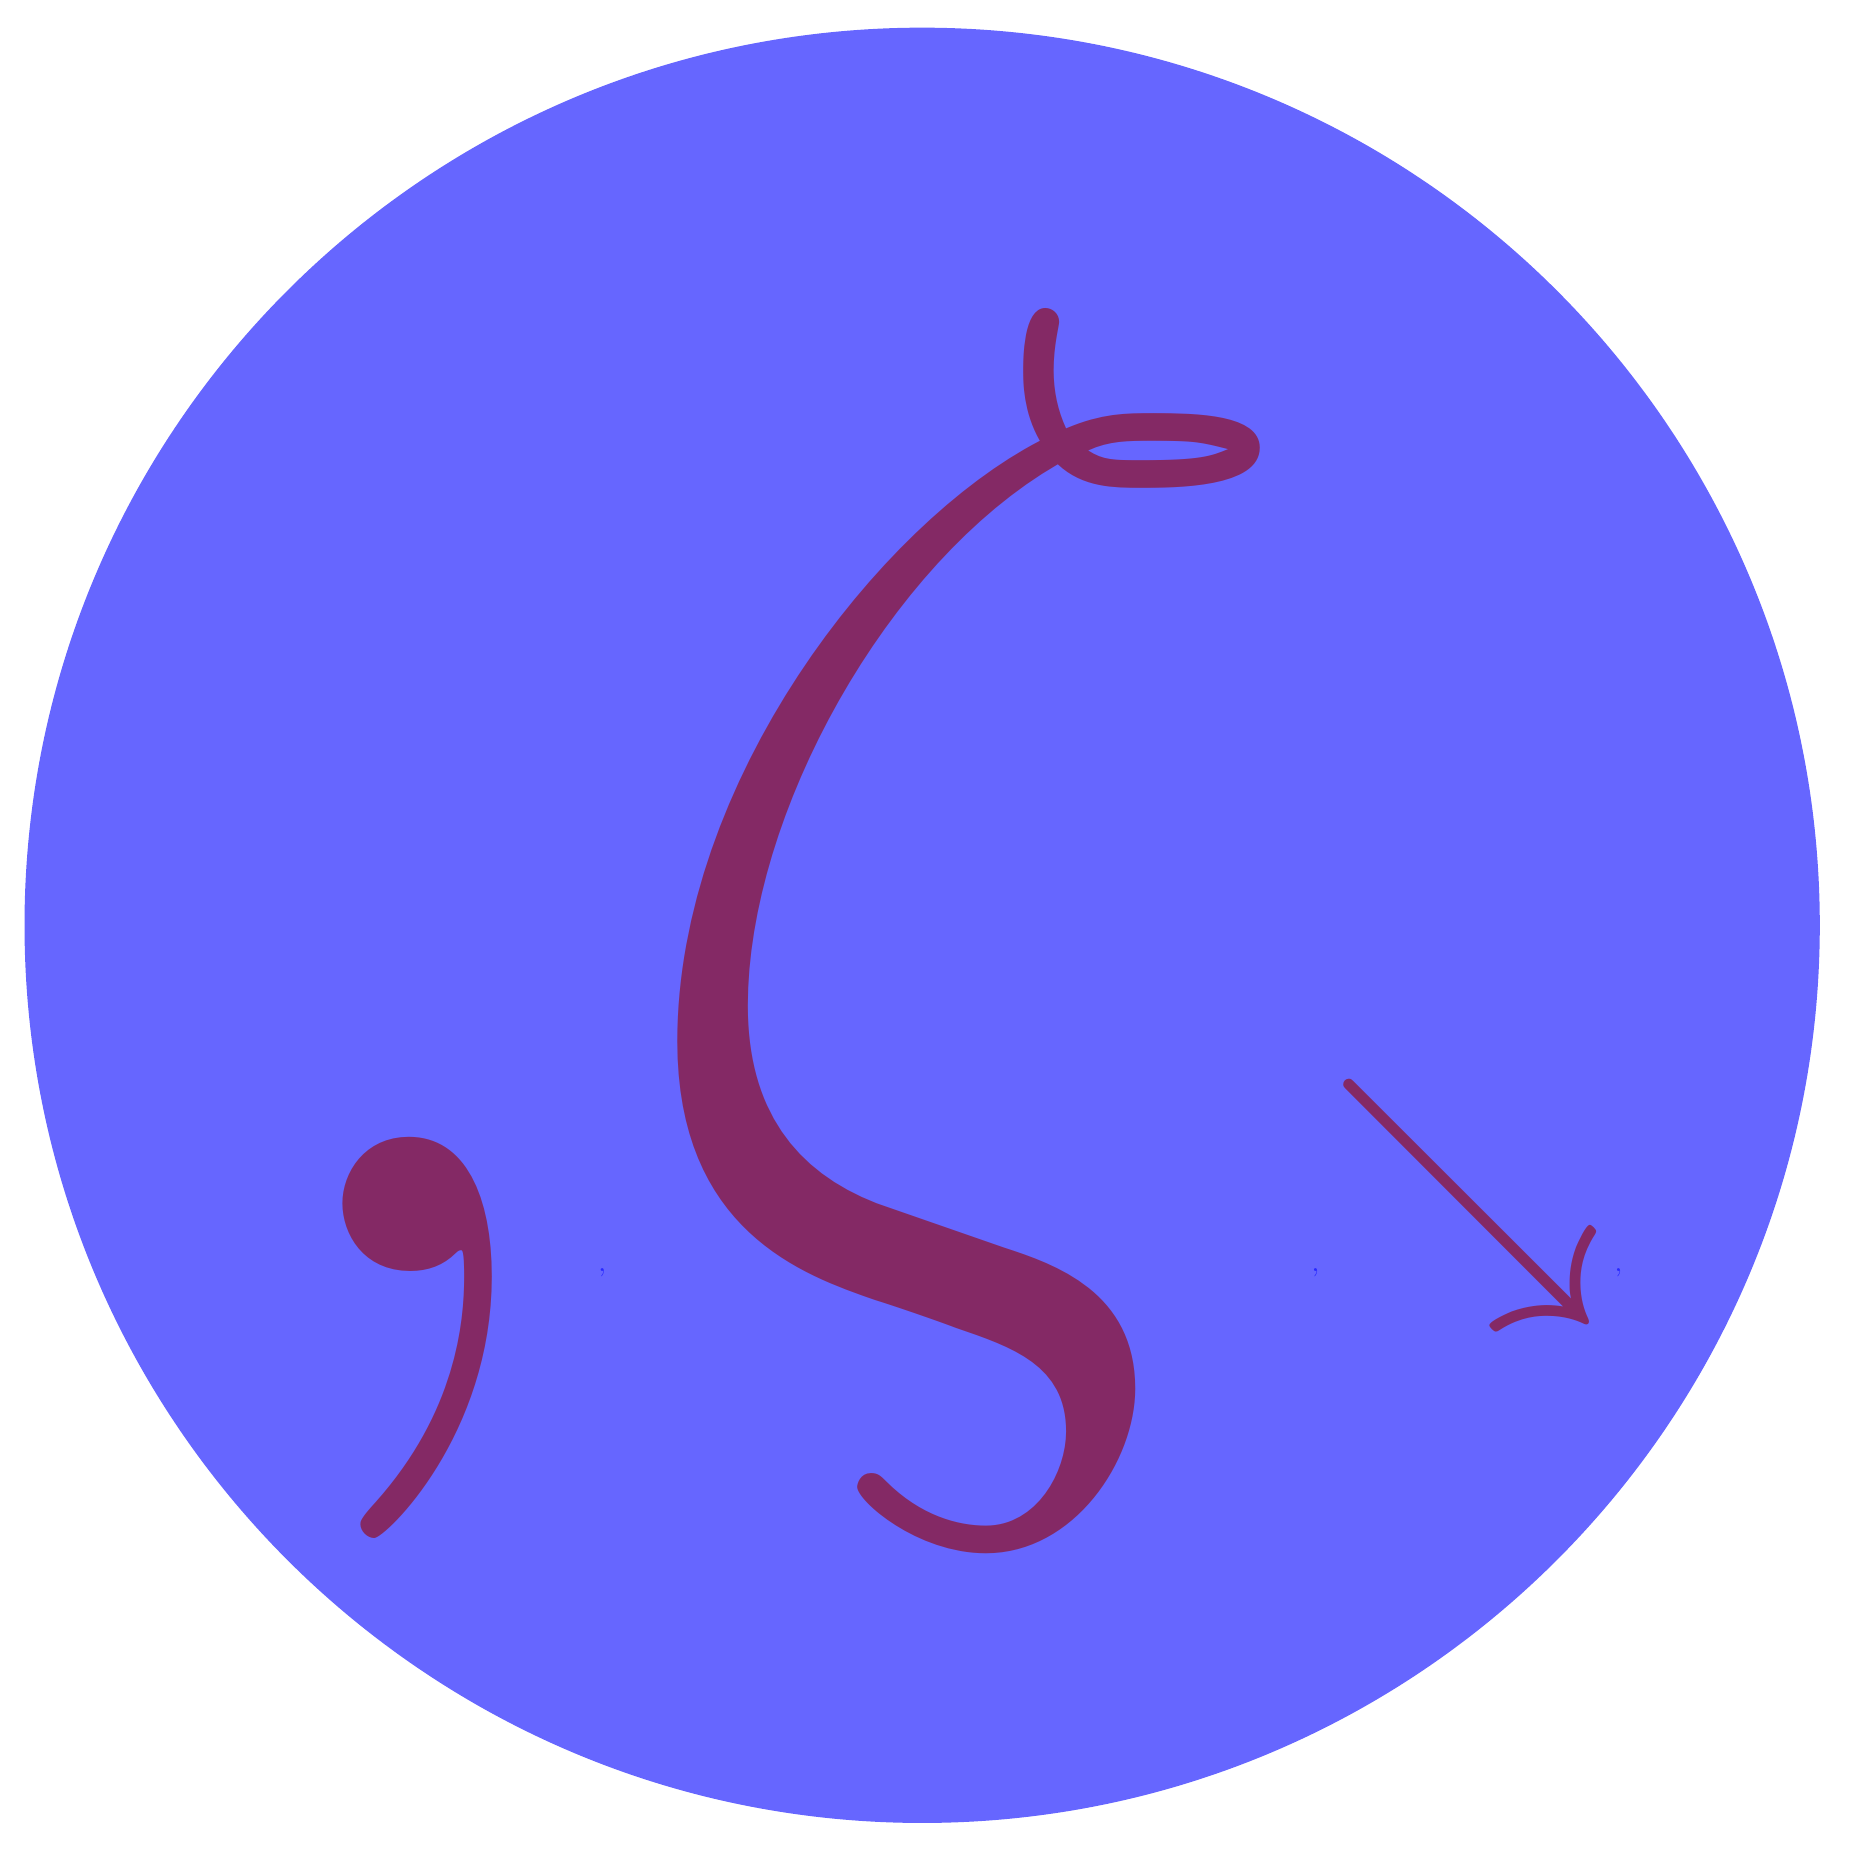
\begin{tikzpicture}
  \coordinate (O) at (0,0) ;
  \coordinate (A) at (0,-2);
  \coordinate (B) at (1.29377,-0.759051);
  \coordinate (C) at (1.53209,-1.28558);

%   \draw [fill=black!90!white](O) circle (11.4cm);
%   \draw [fill=white] (O) circle (7mm);
%   \draw (0,0) node {\fontsize{200}{10}{{\textcolor{red!60!black}{藤田}};
%   \draw (0,0) node {
%       \fontsize{200}{100}{
%         \textcolor{red!60!black}{藤田}
%         }
%     };

  % \fill [blue,opacity=0.6] (0,0) circle (11.4cm) node{\fontsize{100}{10}{
  %   \textcolor{red!60!black}{$\surd$}
  % }};
  \fill [blue,opacity=0.6] (0,0) circle (11.4cm) node{
    \fontsize{500}{10}{\textcolor{red!60!black}{$,$}},
    \fontsize{500}{10}{\textcolor{red!60!black}{$\zeta$}},
    \fontsize{100}{10}{\textcolor{red!60!black}{$\searrow$ }},
            % \textcolor{red!60!black}{$\searrow$}
            };
  
  % \draw [fill=white] (-0.1,-0.1) circle (1.88);
  % \draw (0,0.3) node [anchor=north]{Kontsevich's world};

  % \draw [fill=black] (A) to [out=10,in=-110] (B) to [out=-90,in=200] (C) to [out=-135,in=0] (A); 

%   \foreach \angle / \label in 
%   {
%     0/\fontsize{30}{10}{\textcolor{white}{$\det\!\begin{pmatrix}4&5\\1 &2\end{pmatrix}$}},
%     30/\fontsize{40}{10}{\textcolor{white}{$\displaystyle[\mathbb{C}:\mathbb{R}]$}},
%     60/\fontsize{30}{10}{\textcolor{white}{$\displaystyle\lim_{x\rightarrow 0}\frac{\sin x}{x}$}},
%     90/\fontsize{50}{10}{\textcolor{white}{$\frac{2\pi^2}{\zeta(2)}$}},
%     120/\fontsize{35}{10}{\textcolor{white}{$\displaystyle\sqrt{121}$}},
%     150/\fontsize{35}{10}{\textcolor{white}{$\displaystyle|E(W_6)|$}},
%     180/\fontsize{35}{10}{\textcolor{white}{$\displaystyle\pi(25)$}},
%     210/\fontsize{25}{10}{\textcolor{white}{$\hspace{30mm}\displaystyle\us\iiint_{|x|+|y|+|z|\leq 1}\hspace{-10mm}6dxdydz$}},
%     240/\fontsize{35}{10}{\textcolor{white}{$\displaystyle\dim_\mathbb{Q}\mathcal{Z}_{10}$}},
%     270/\fontsize{50}{10}{\textcolor{white}{$\#\mathfrak{S}_3$}},
%     300/\fontsize{35}{10}{\textcolor{white}{$\displaystyle(2\phi -1)^2$}},
%     330/\fontsize{30}{10}{\textcolor{white}{$\displaystyle\gcd(2020,32)\ \ \ \ \ \ \ \ \ $}}
%   } 
%   { 
%   %  \draw (\angle:22cm) -- (\angle:12cm); 
%    \node at (\angle:9cm) {\textsf{\label}}; 
%   } 

\end{tikzpicture}
% \end{center}
    %時計の例(2変数指定の例)
    % \begin{tikzpicture}
    % \draw[very thick] (0,0) circle (2cm);%時計の外周
    % \foreach \angle / \label in 
    %   {0/$\cdot$, 15/$\cdot$, 30/$\cdot$, 45/$\cdot$, 60/$\cdot$,75/$\cdot$, 90/$\cdot$, 
    %   105/$\cdot$, 120/$\cdot$, 135/$\cdot$, 150/$\cdot$, 165/$\cdot$,
    %   180/$\cdot$, 190/\rotatebox{-80}{$>$}, 205/$2$, 220/\rotatebox{-50}{$>$}, 235/$1$, 
    %   250/\rotatebox{-20}{$>$}, 270/$0\equiv p$, 290/\rotatebox{20}{$>$}, 305/$\ \ p-1$, 
    %   320/\rotatebox{50}{$>$}, 335/$\ \ p-2$} 
    %   { 
    % %    \draw (\angle:1.8cm) -- (\angle:2cm); 
    %    \node at (\angle:2.5cm) {\textsf{\label}}; 
    %   } 
    % % \foreach \angle in {0,90,180,270} 
    % %    \draw[thick] (\angle:1.7cm) -- (\angle:2cm); 
    % % \draw[line width=3pt, cap=round] (0,0) -- (145:0.8cm);%短針
    % % \draw[line width=3pt, cap=round] (0,0) -- (30:1.2cm);%長針
    % \end{tikzpicture}


    %黒青色のやつ
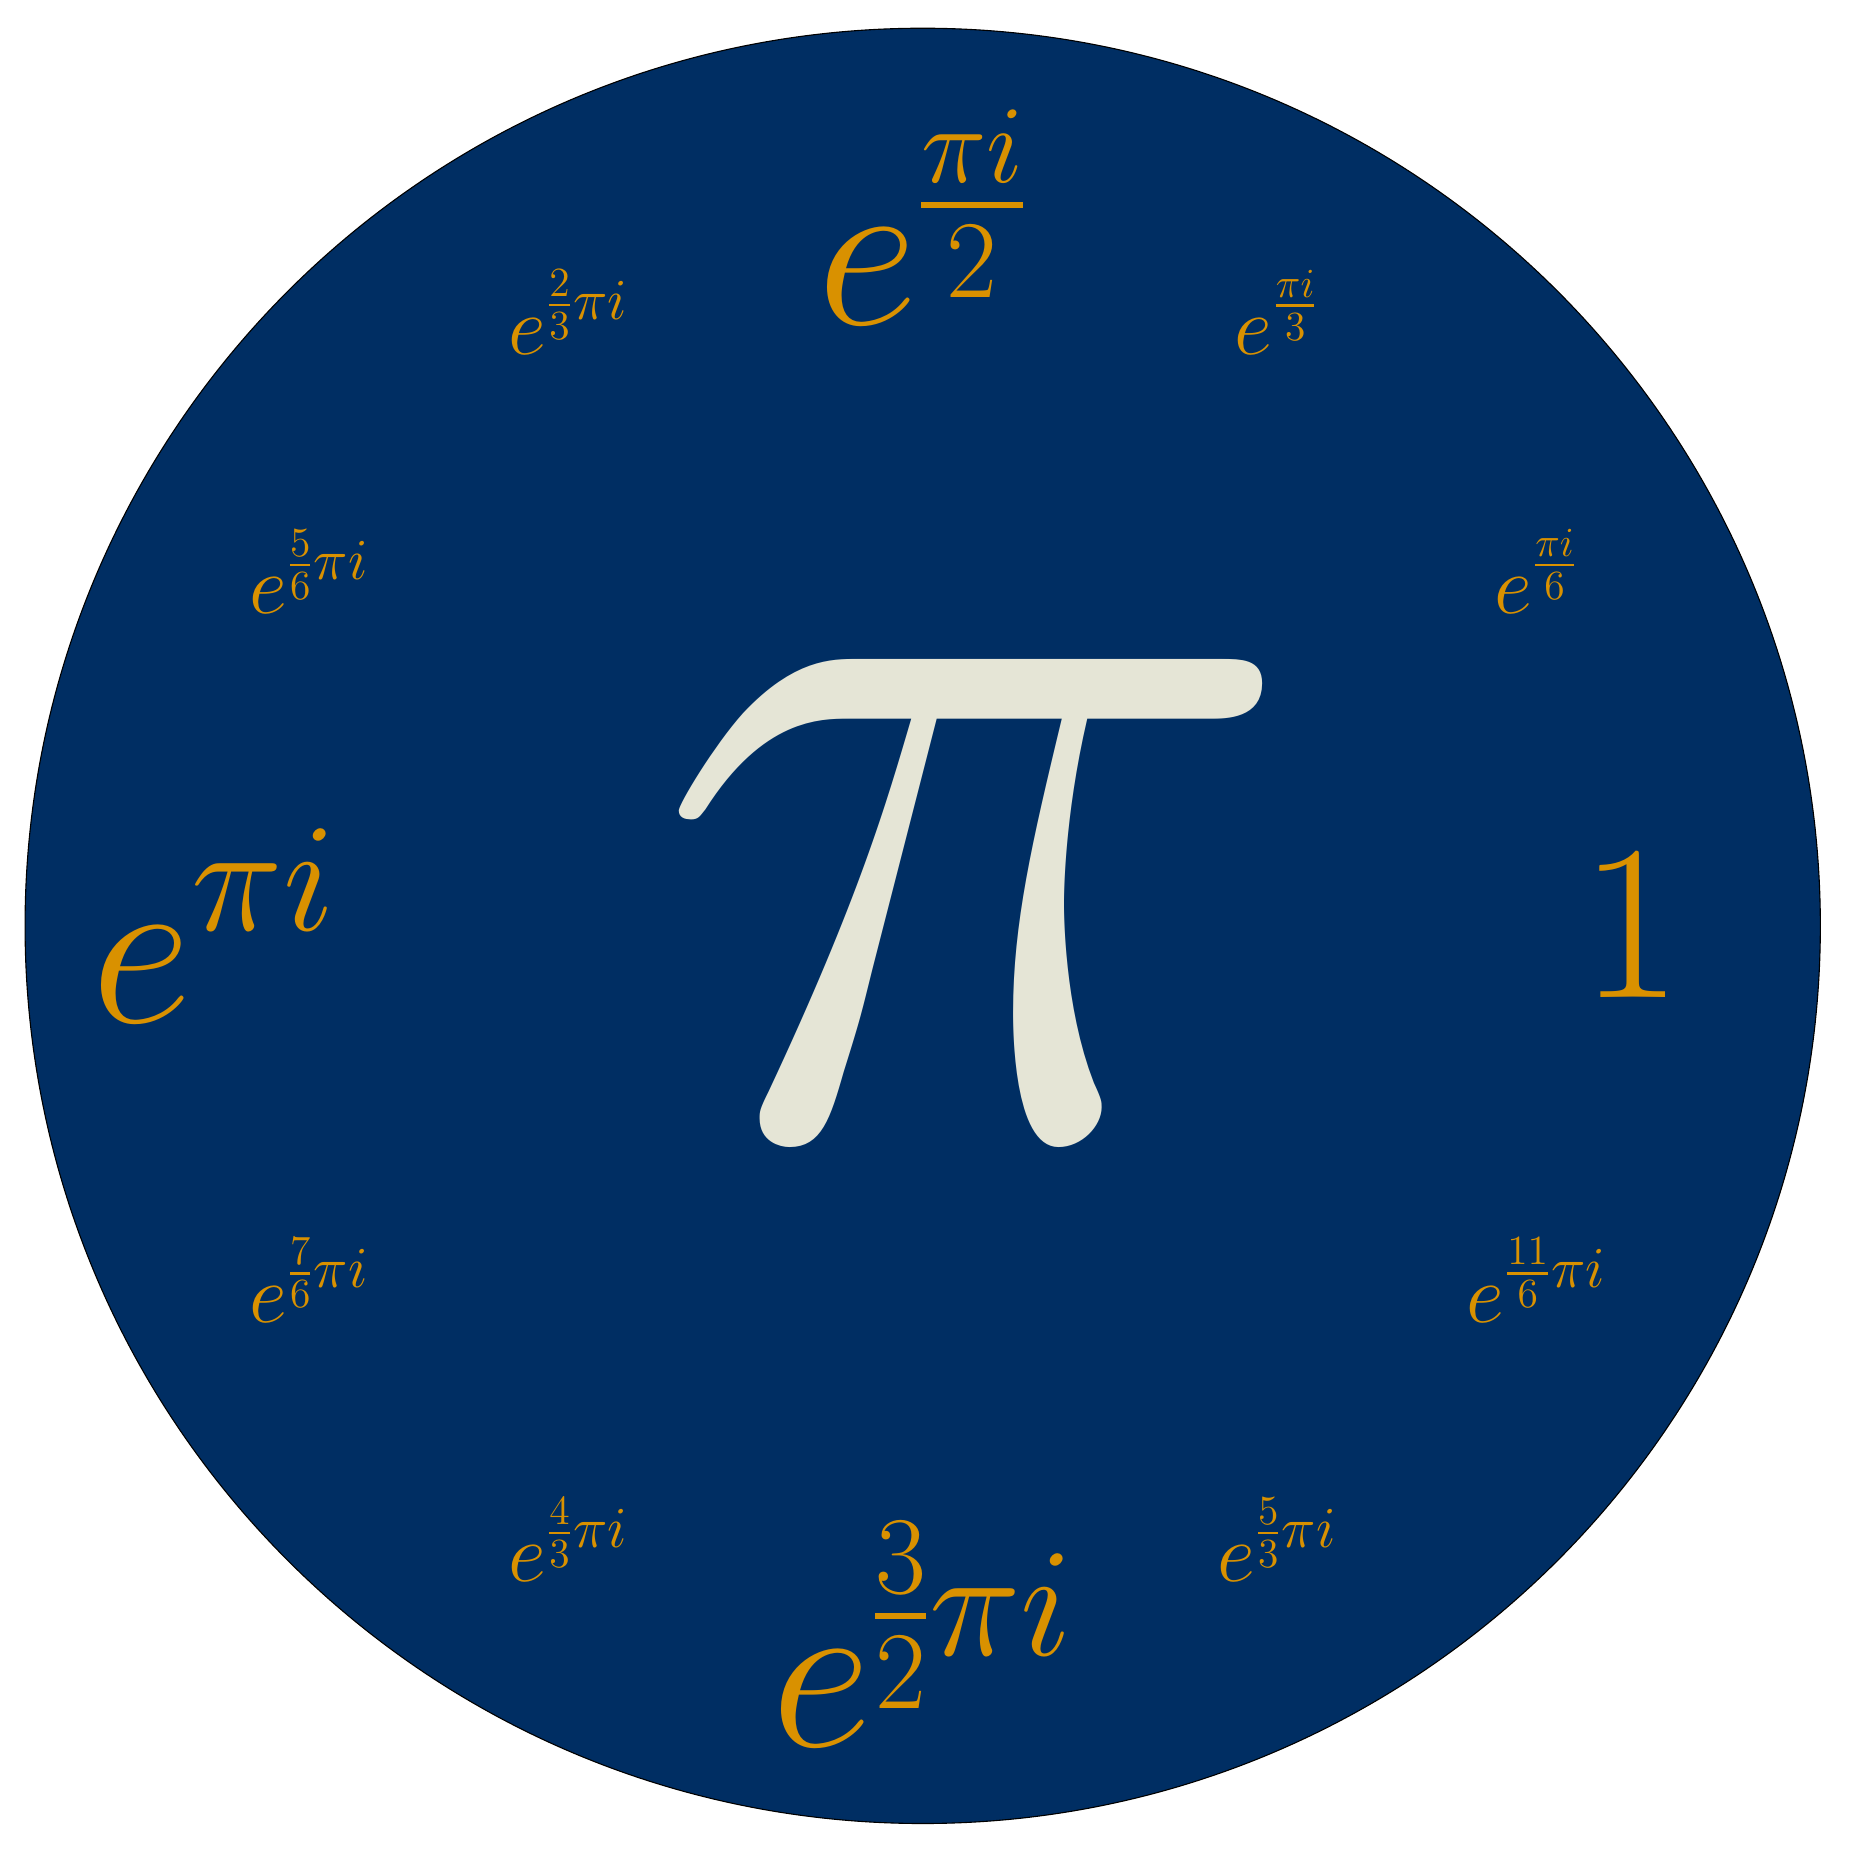
\begin{tikzpicture}
  \coordinate (O) at (0,0);
  \coordinate (A) at (0,-2);
  \coordinate (B) at (1.29377,-0.759051);
  \coordinate (C) at (1.53209,-1.28558);

  \draw [fill=coolblack](O) circle (11.4cm);
  % \draw [fill=white] (O) circle (7mm);
  % \draw (0,-2) node [anchor=north]{\fontsize{20}{10}{\textit{\textcolor{red!60!black}{Mathematics with \TeX}}}};
  \draw (0.7,3.5) node [anchor=north]{\fontsize{20}{10}{\textit{\textcolor{ivory}{{\fontsize{400pt}{400pt}\selectfont $\displaystyle \pi$}}}}};

  \foreach \angle / \label in 
  {
    0/\fontsize{80}{10}{\textcolor{harvestgold}{$1$}},
    30/\fontsize{30}{10}{\textcolor{harvestgold}{$\displaystyle  e^{\frac{\pi i}{6}}$}},
    60/\fontsize{30}{10}{\textcolor{harvestgold}{$\displaystyle e^{\frac{\pi i}{3}}$}},
    90/\fontsize{80}{10}{\textcolor{harvestgold}{$e^{\frac{\pi i}{2}}$}},
    120/\fontsize{30}{10}{\textcolor{harvestgold}{$\displaystyle e^{\frac{2}{3}\pi i}$}},
    150/\fontsize{30}{10}{\textcolor{harvestgold}{$\displaystyle e^{\frac{5}{6}\pi i}$}},
    180/\fontsize{80}{10}{\textcolor{harvestgold}{$\displaystyle e^{\pi i}$}},
    210/\fontsize{30}{10}{\textcolor{harvestgold}{$\displaystyle e^{\frac{7}{6}\pi i}$}},
    240/\fontsize{30}{10}{\textcolor{harvestgold}{$\displaystyle e^{\frac{4}{3}\pi i}$}},
    270/\fontsize{80}{10}{\textcolor{harvestgold}{$\displaystyle e^{\frac{3}{2}\pi i}$}},
    300/\fontsize{30}{10}{\textcolor{harvestgold}{$\displaystyle e^{\frac{5}{3}\pi i}$}},
    330/\fontsize{30}{10}{\textcolor{harvestgold}{$\displaystyle e^{\frac{11}{6}\pi i}$}}
  } 
  { 
  %  \draw (\angle:22cm) -- (\angle:12cm); 
   \node at (\angle:9cm) {\textsf{\label}}; 
  } 

\end{tikzpicture}

    %薄青色のやつ
    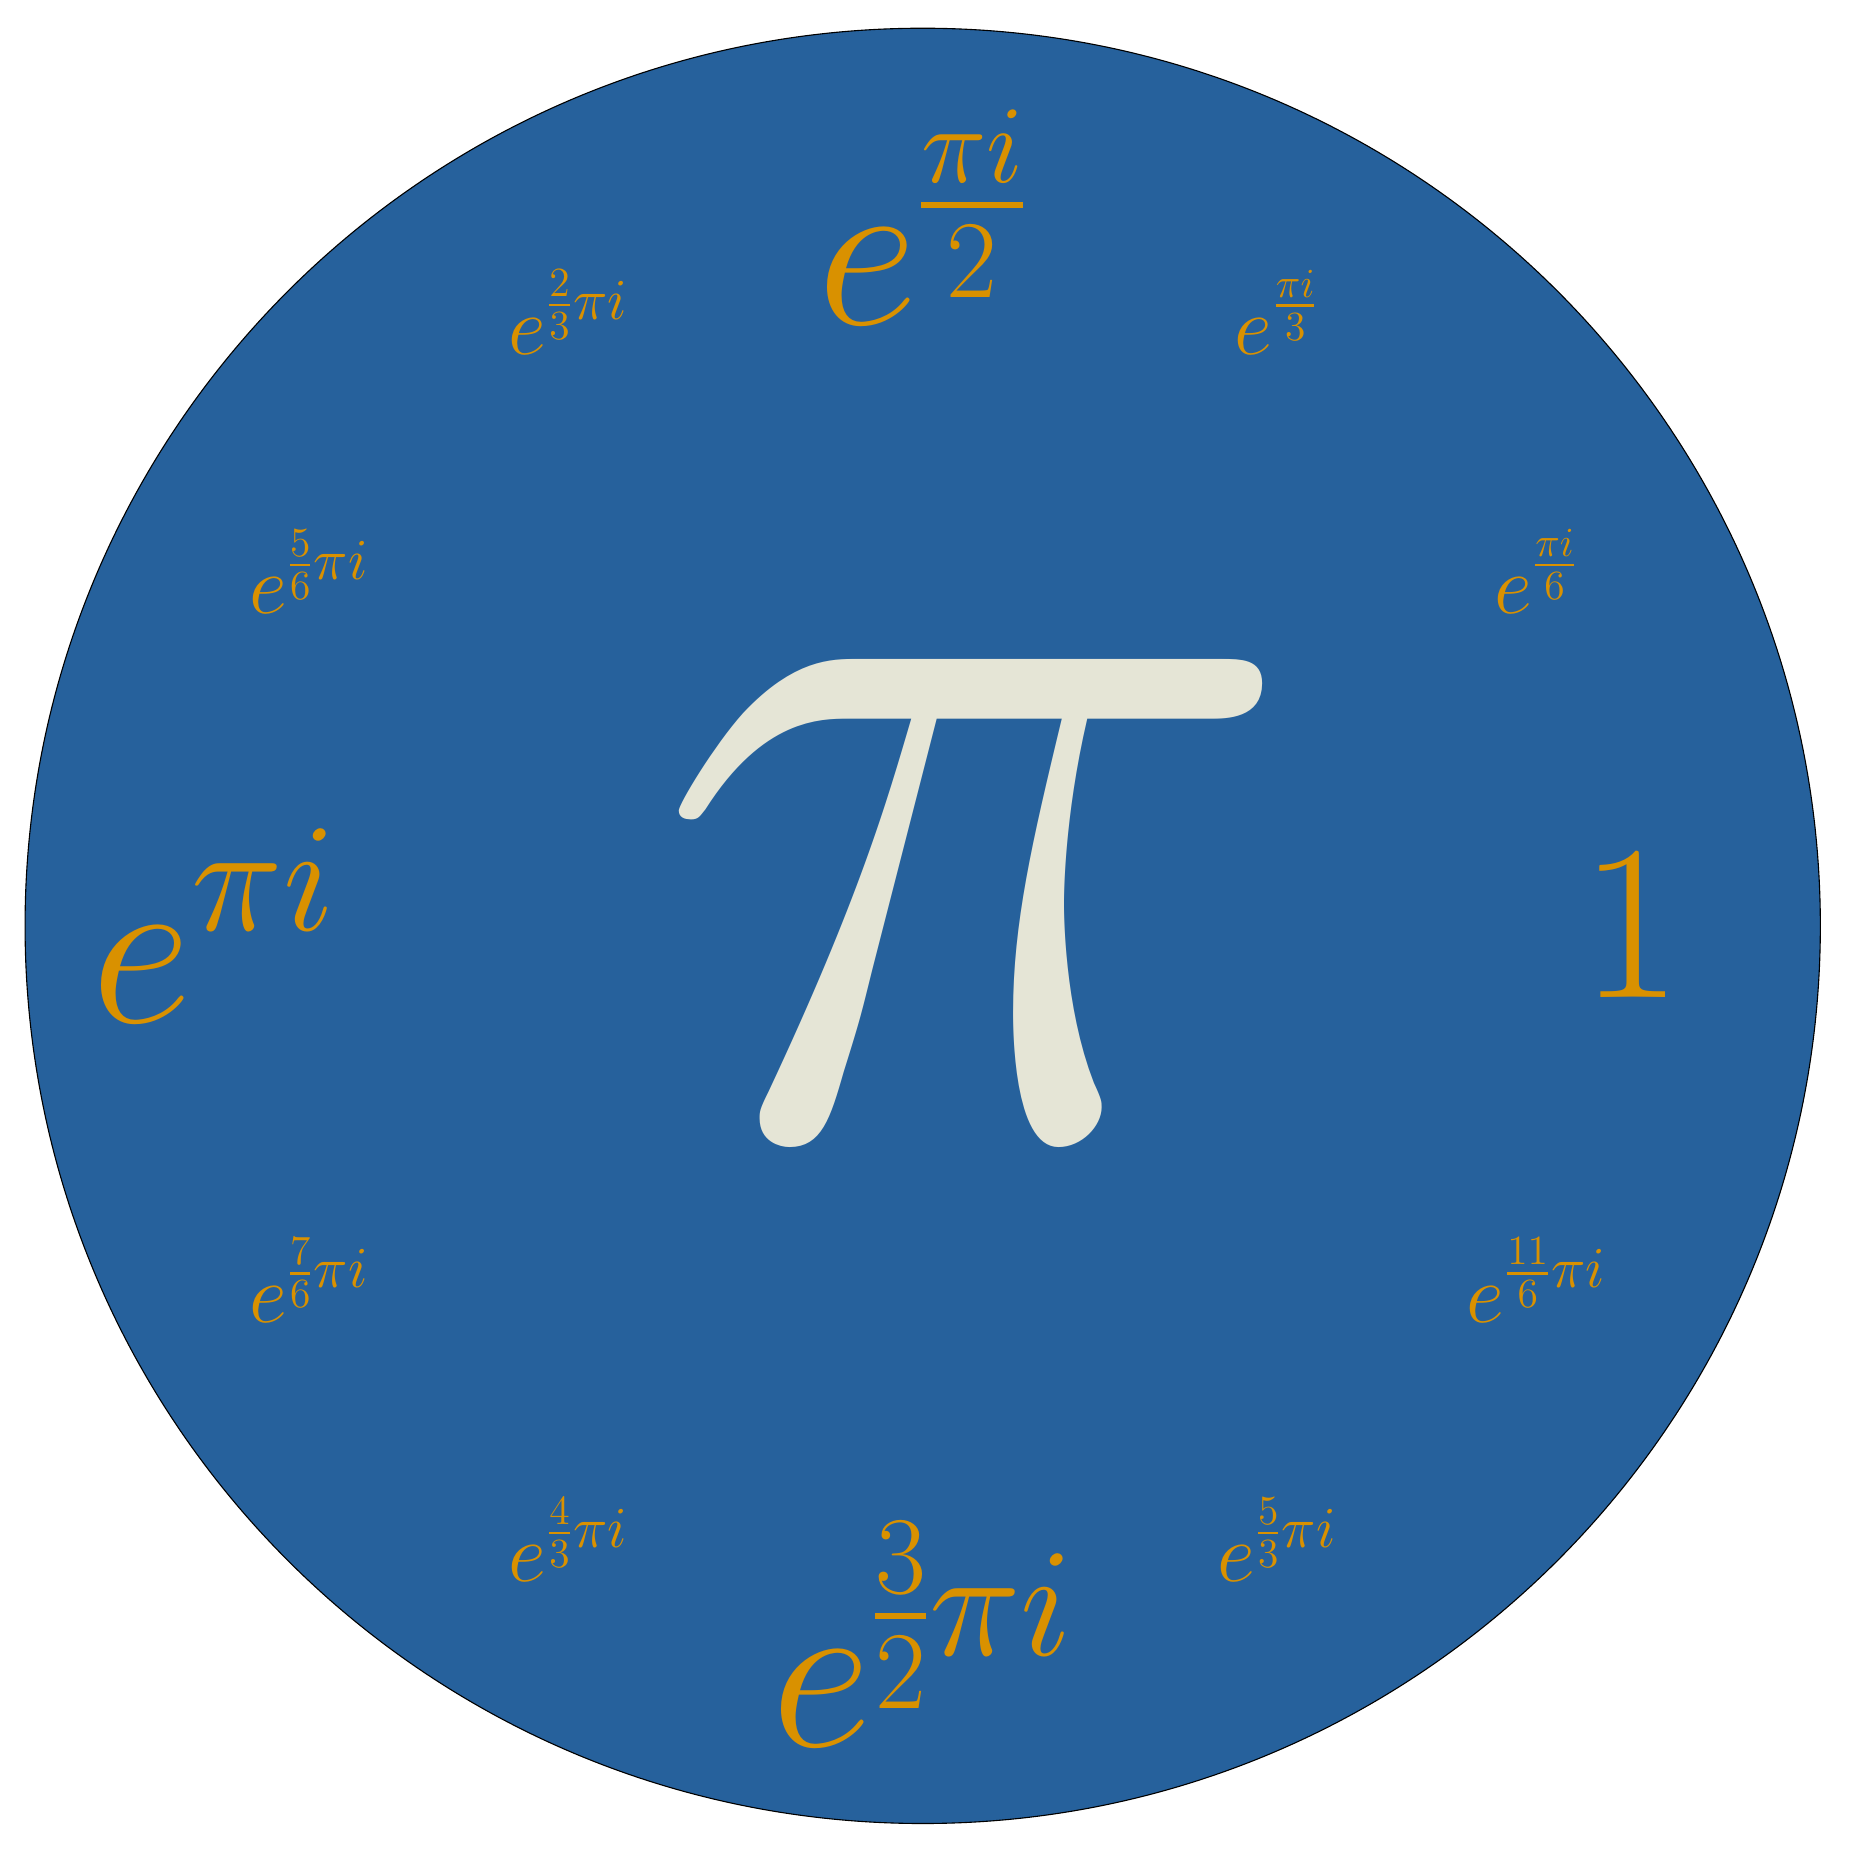
\begin{tikzpicture}
      \coordinate (O) at (0,0);
      \coordinate (A) at (0,-2);
      \coordinate (B) at (1.29377,-0.759051);
      \coordinate (C) at (1.53209,-1.28558);
    
      \draw [fill=lapislazuli](O) circle (11.4cm);
      % \draw [fill=white] (O) circle (7mm);
      % \draw (0,-2) node [anchor=north]{\fontsize{20}{10}{\textit{\textcolor{red!60!black}{Mathematics with \TeX}}}};
      \draw (0.7,3.5) node [anchor=north]{\fontsize{20}{10}{\textit{\textcolor{ivory}{{\fontsize{400pt}{400pt}\selectfont $\displaystyle \pi$}}}}};
    
      \foreach \angle / \label in 
      {
        0/\fontsize{80}{10}{\textcolor{harvestgold}{$1$}},
        30/\fontsize{30}{10}{\textcolor{harvestgold}{$\displaystyle  e^{\frac{\pi i}{6}}$}},
        60/\fontsize{30}{10}{\textcolor{harvestgold}{$\displaystyle e^{\frac{\pi i}{3}}$}},
        90/\fontsize{80}{10}{\textcolor{harvestgold}{$e^{\frac{\pi i}{2}}$}},
        120/\fontsize{30}{10}{\textcolor{harvestgold}{$\displaystyle e^{\frac{2}{3}\pi i}$}},
        150/\fontsize{30}{10}{\textcolor{harvestgold}{$\displaystyle e^{\frac{5}{6}\pi i}$}},
        180/\fontsize{80}{10}{\textcolor{harvestgold}{$\displaystyle e^{\pi i}$}},
        210/\fontsize{30}{10}{\textcolor{harvestgold}{$\displaystyle e^{\frac{7}{6}\pi i}$}},
        240/\fontsize{30}{10}{\textcolor{harvestgold}{$\displaystyle e^{\frac{4}{3}\pi i}$}},
        270/\fontsize{80}{10}{\textcolor{harvestgold}{$\displaystyle e^{\frac{3}{2}\pi i}$}},
        300/\fontsize{30}{10}{\textcolor{harvestgold}{$\displaystyle e^{\frac{5}{3}\pi i}$}},
        330/\fontsize{30}{10}{\textcolor{harvestgold}{$\displaystyle e^{\frac{11}{6}\pi i}$}}
      } 
      { 
      %  \draw (\angle:22cm) -- (\angle:12cm); 
       \node at (\angle:9cm) {\textsf{\label}}; 
      } 
    
    \end{tikzpicture}



        %黒緑色のやつ
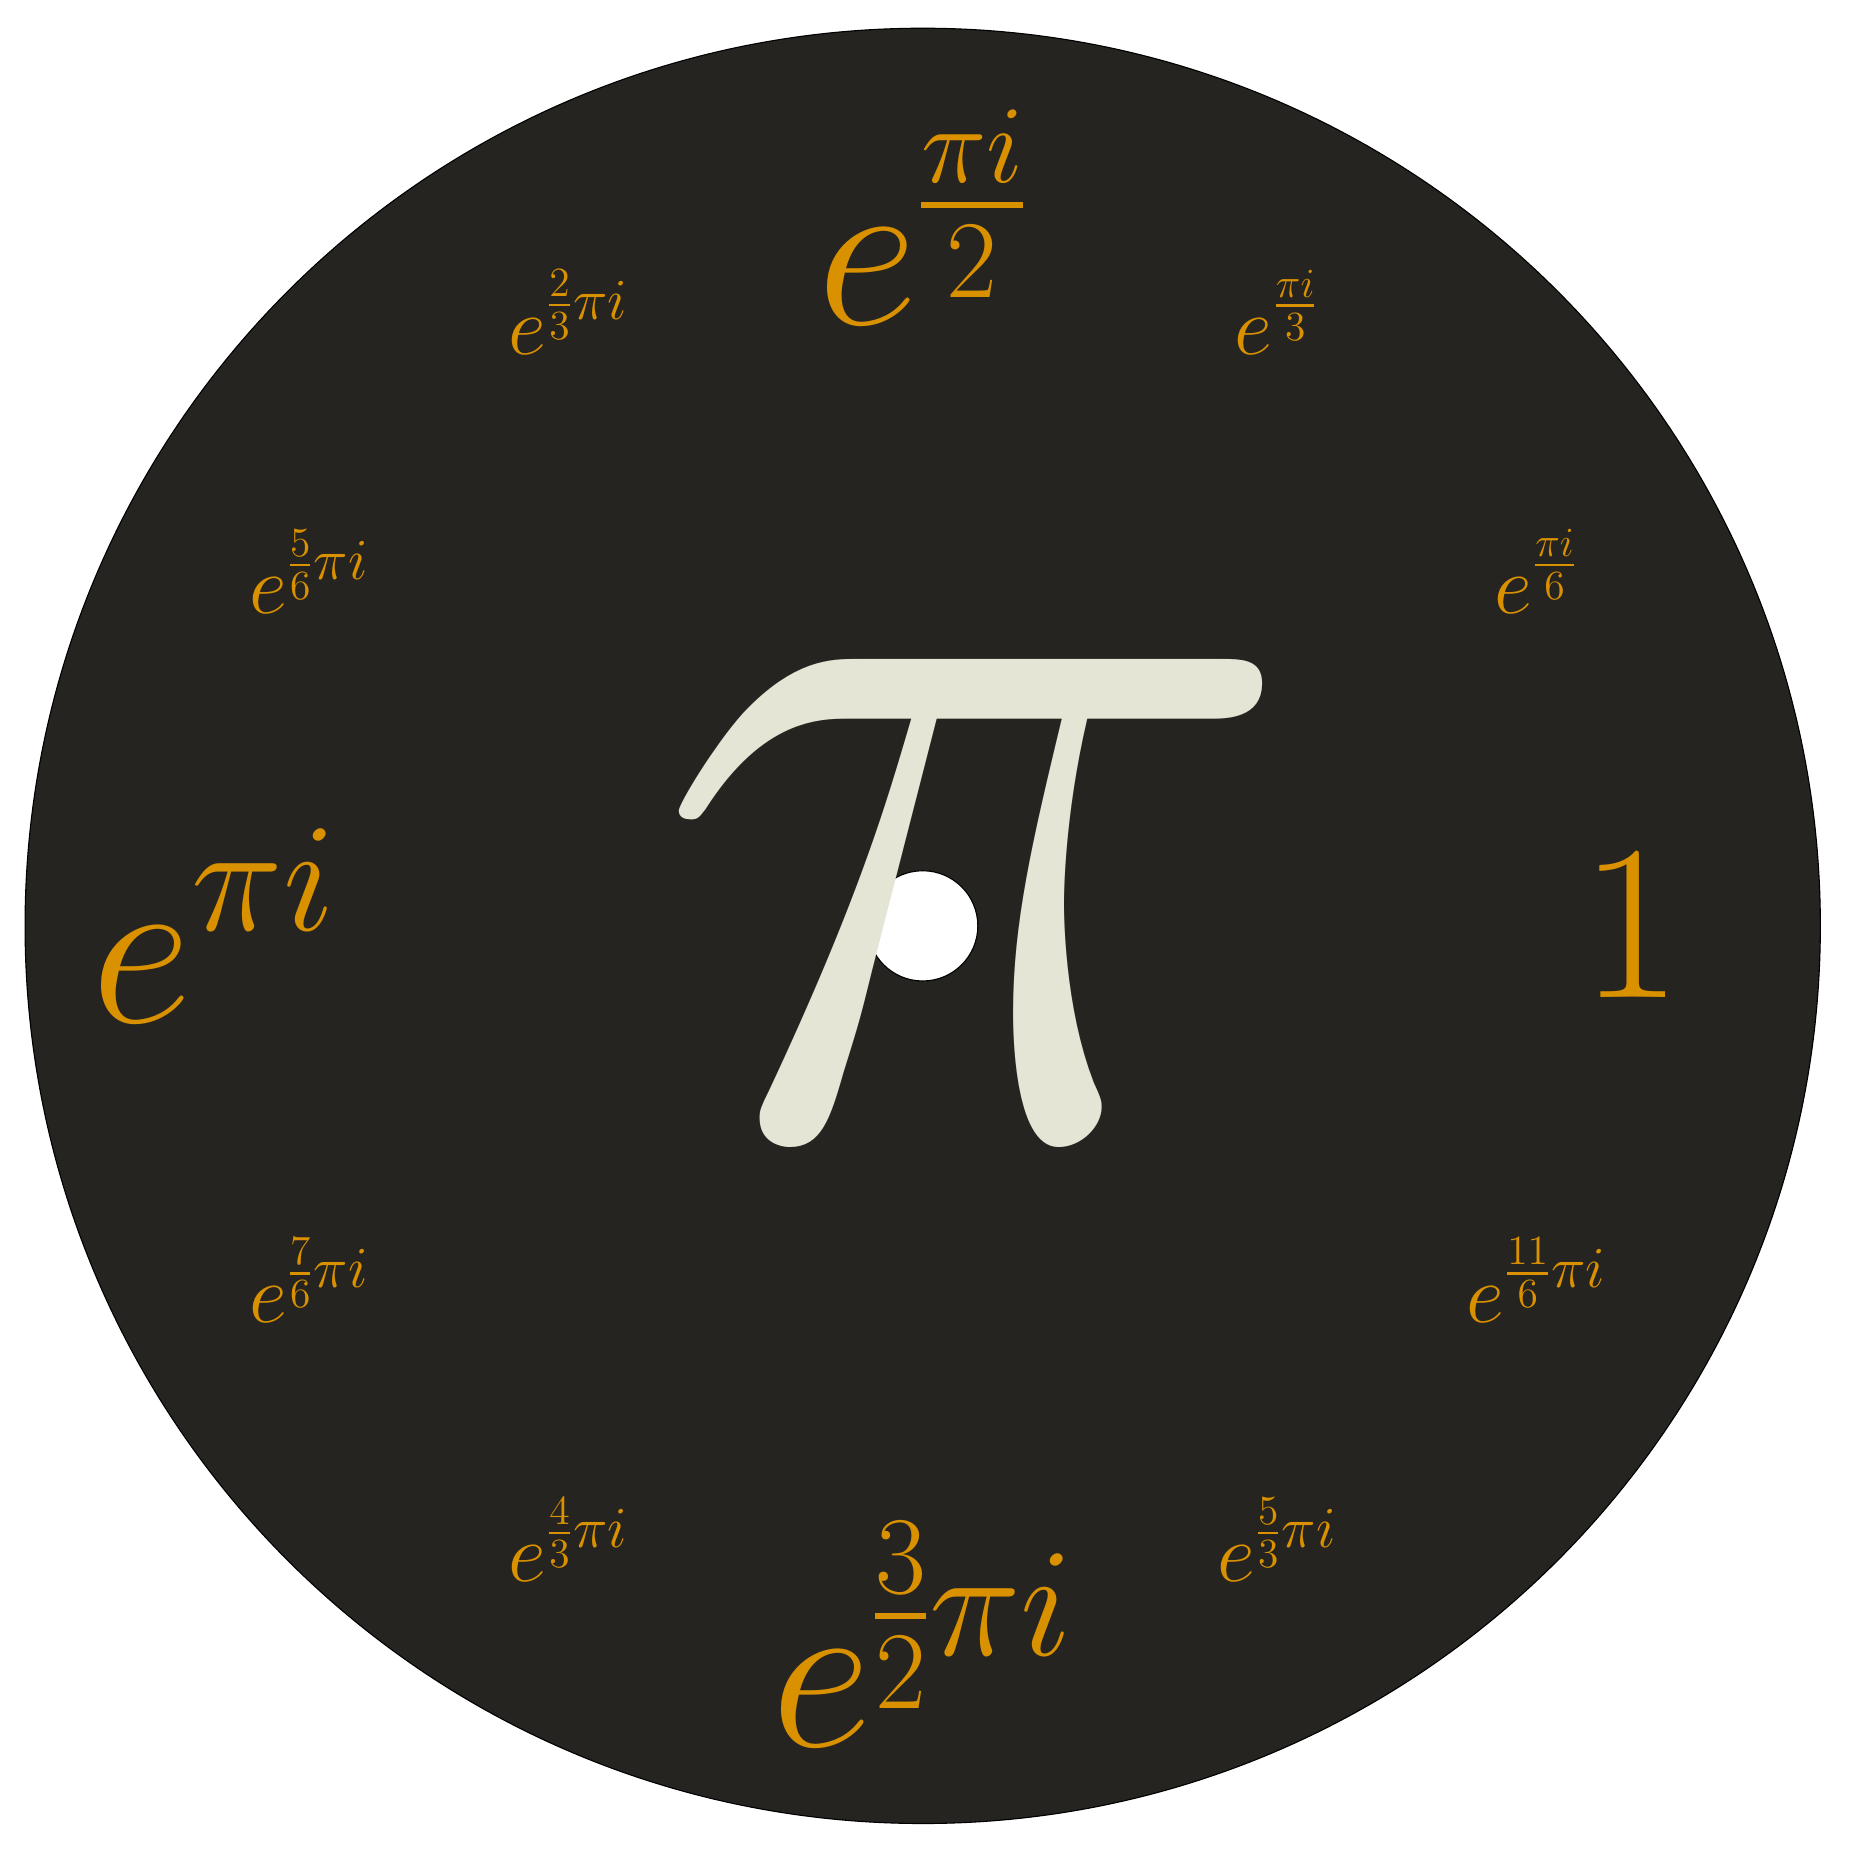
\begin{tikzpicture}
  \coordinate (O) at (0,0);
  \coordinate (A) at (0,-2);
  \coordinate (B) at (1.29377,-0.759051);
  \coordinate (C) at (1.53209,-1.28558);

  \draw [fill=darkjunglegreen](O) circle (11.4cm);
  % \draw [fill=deepjunglegreen](O) circle (11.4cm);
  % \draw [fill=mediumjunglegreen](O) circle (11.4cm);
  \draw [fill=white] (O) circle (7mm);
  % \draw (0,-2) node [anchor=north]{\fontsize{20}{10}{\textit{\textcolor{red!60!black}{Mathematics with \TeX}}}};
  \draw (0.7,3.5) node [anchor=north]{\fontsize{20}{10}{\textit{\textcolor{ivory}{{\fontsize{400pt}{400pt}\selectfont $\displaystyle \pi$}}}}};

  \foreach \angle / \label in 
  {
    0/\fontsize{80}{10}{\textcolor{harvestgold}{$1$}},
    30/\fontsize{30}{10}{\textcolor{harvestgold}{$\displaystyle  e^{\frac{\pi i}{6}}$}},
    60/\fontsize{30}{10}{\textcolor{harvestgold}{$\displaystyle e^{\frac{\pi i}{3}}$}},
    90/\fontsize{80}{10}{\textcolor{harvestgold}{$e^{\frac{\pi i}{2}}$}},
    120/\fontsize{30}{10}{\textcolor{harvestgold}{$\displaystyle e^{\frac{2}{3}\pi i}$}},
    150/\fontsize{30}{10}{\textcolor{harvestgold}{$\displaystyle e^{\frac{5}{6}\pi i}$}},
    180/\fontsize{80}{10}{\textcolor{harvestgold}{$\displaystyle e^{\pi i}$}},
    210/\fontsize{30}{10}{\textcolor{harvestgold}{$\displaystyle e^{\frac{7}{6}\pi i}$}},
    240/\fontsize{30}{10}{\textcolor{harvestgold}{$\displaystyle e^{\frac{4}{3}\pi i}$}},
    270/\fontsize{80}{10}{\textcolor{harvestgold}{$\displaystyle e^{\frac{3}{2}\pi i}$}},
    300/\fontsize{30}{10}{\textcolor{harvestgold}{$\displaystyle e^{\frac{5}{3}\pi i}$}},
    330/\fontsize{30}{10}{\textcolor{harvestgold}{$\displaystyle e^{\frac{11}{6}\pi i}$}}
  } 
  { 
  %  \draw (\angle:22cm) -- (\angle:12cm); 
   \node at (\angle:9cm) {\textsf{\label}}; 
  } 

\end{tikzpicture}


    %Kontsevich's order
    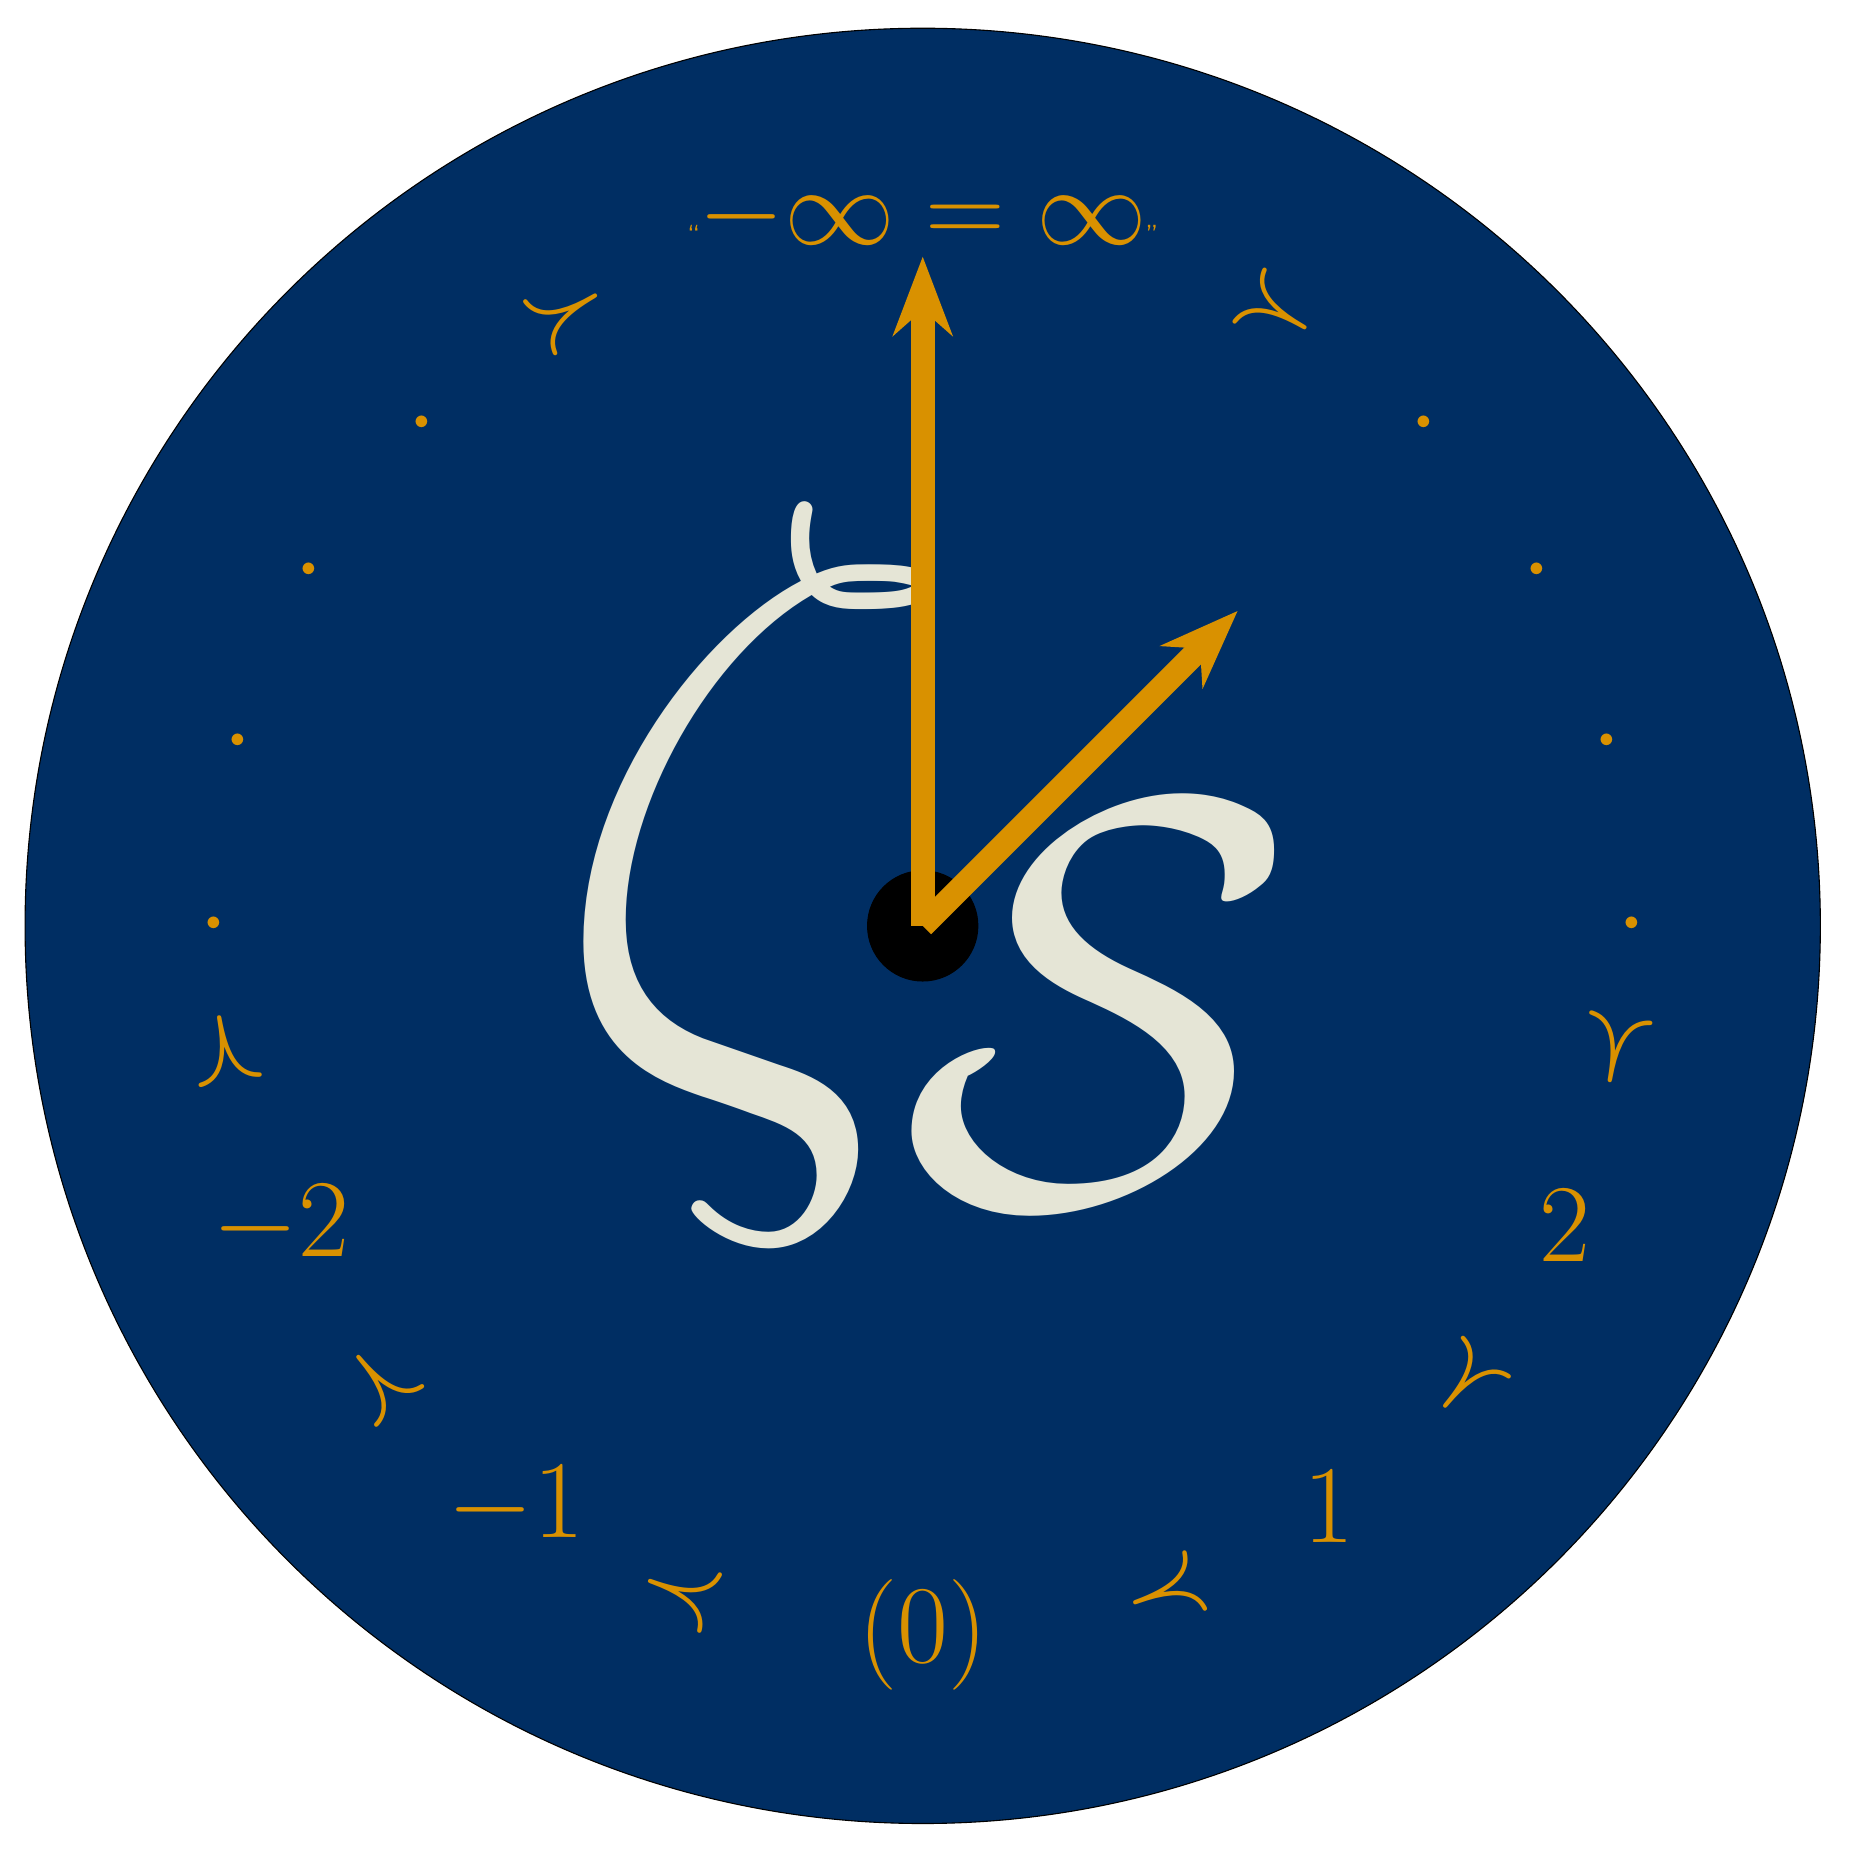
\begin{tikzpicture}
      \coordinate (O) at (0,0);
      \coordinate (OO) at (0,5.5);
      \coordinate (A) at (0,-2);
      \coordinate (B) at (1.29377,-0.759051);
      \coordinate (C) at (1.53209,-1.28558);
    
      \draw [fill=coolblack](O) circle (11.4cm);
      \draw [fill=black] (O) circle (7mm);
      % \draw (0,-2) node [anchor=north]{\fontsize{20}{10}{\textit{\textcolor{red!60!black}{Mathematics with \TeX}}}};
      \draw (OO) node [anchor=north]{\fontsize{20}{10}{\textit{\textcolor{ivory}{{\fontsize{300pt}{300pt}\selectfont $\displaystyle \zeta_\mathcal{S}$}}}}};
      \draw [harvestgold,line width=3mm, -{Stealth[length=10mm, open]}] (O) -- (0,8.5);
      \draw [harvestgold,line width=3mm, -{Stealth[length=10mm, open]}] (O) -- (4,4);
      \foreach \angle / \label in 
      {
        % 0/\fontsize{50}{10}{\textcolor{harvestgold}{\rotatebox{90}{$\prec$}}},
        % 30/\fontsize{50}{10}{\textcolor{harvestgold}{\rotatebox{120}{$\cdots$}}},
        % % 60/\fontsize{50}{10}{\textcolor{harvestgold}{$f$}},
        % 90/\fontsize{50}{10}{\textcolor{harvestgold}{$(-\infty=\infty)$}},
        % % 120/\fontsize{50}{10}{\textcolor{harvestgold}{$f$}},
        % 150/\fontsize{50}{10}{\textcolor{harvestgold}{$f$}},
        % 180/\fontsize{50}{10}{\textcolor{harvestgold}{\rotatebox{90}{$\prec$}}},
        % 210/\fontsize{50}{10}{\textcolor{harvestgold}{$\displaystyle -1$}},
        % 240/\fontsize{50}{10}{\textcolor{harvestgold}{\rotatebox{-30}{$\prec$}}},
        % 270/\fontsize{50}{10}{\textcolor{harvestgold}{$\displaystyle (0)$}},
        % 300/\fontsize{50}{10}{\textcolor{harvestgold}{\rotatebox{30}{$\prec$}}},
        % 330/\fontsize{50}{10}{\textcolor{harvestgold}{$\displaystyle 1$}}
        % 
        % 0/$\cdot$, 15/$\cdot$, 30/$\cdot$, 45/$\cdot$, 60/$\cdot$,75/$\cdot$, 90/$\cdot$, 
        % 105/$\cdot$, 120/$\cdot$, 135/$\cdot$, 150/$\cdot$, 165/$\cdot$,
        % 180/$\cdot$, 190/\rotatebox{100}{$>$}, 205/$p-2\ $, 220/\rotatebox{130}{$>$}, 235/$p-1\ $, 
        % 250/\rotatebox{160}{$>$}, 270/$p\equiv 0$, 290/\rotatebox{200}{$>$}, 305/$\ \ 1$, 
        % 320/\rotatebox{230}{$>$}, 335/$\ \ 2$, 350/\rotatebox{260}{$>$}
        % 
        0/\fontsize{40}{10}{\textcolor{harvestgold}{$\cdot$}}, 
        15/\fontsize{40}{10}{\textcolor{harvestgold}{$\cdot$}}, 
        30/\fontsize{40}{10}{\textcolor{harvestgold}{$\cdot$}}, 
        45/\fontsize{40}{10}{\textcolor{harvestgold}{$\cdot$}}, 
        60/\fontsize{40}{10}{\textcolor{harvestgold}{\rotatebox{150}{$\prec$}}}, 
        90/\fontsize{40}{10}{\textcolor{harvestgold}{``$-\infty=\infty$''}}, 
        120/\fontsize{40}{10}{\textcolor{harvestgold}{\rotatebox{-150}{$\prec$}}},
        135/\fontsize{40}{10}{\textcolor{harvestgold}{$\cdot$}}, 
        150/\fontsize{40}{10}{\textcolor{harvestgold}{$\cdot$}}, 
        165/\fontsize{40}{10}{\textcolor{harvestgold}{$\cdot$}},
        180/\fontsize{40}{10}{\textcolor{harvestgold}{$\cdot$}}, 
        190/\fontsize{40}{10}{\textcolor{harvestgold}{\rotatebox{-80}{$\prec$}}}, 
        205/\fontsize{40}{10}{\textcolor{harvestgold}{$-2$}}, 
        220/\fontsize{40}{10}{\textcolor{harvestgold}{\rotatebox{-50}{$\prec$}}}, 
        235/\fontsize{40}{10}{\textcolor{harvestgold}{$-1$}}, 
        250/\fontsize{40}{10}{\textcolor{harvestgold}{\rotatebox{-20}{$\prec$}}}, 
        270/\fontsize{40}{10}{\textcolor{harvestgold}{$(0)$}}, 
        290/\fontsize{40}{10}{\textcolor{harvestgold}{\rotatebox{20}{$\prec$}}}, 
        305/\fontsize{40}{10}{\textcolor{harvestgold}{$1$}}, 
        320/\fontsize{40}{10}{\textcolor{harvestgold}{\rotatebox{50}{$\prec$}}}, 
        335/\fontsize{40}{10}{\textcolor{harvestgold}{$2$}}, 
        350/\fontsize{40}{10}{\textcolor{harvestgold}{\rotatebox{80}{$\prec$}}
        }
      } 
      { 
      %  \draw (\angle:22cm) -- (\angle:12cm); 
       \node at (\angle:9cm) {\textsf{\label}}; 
      } 
    \end{tikzpicture}
    
    %p order
    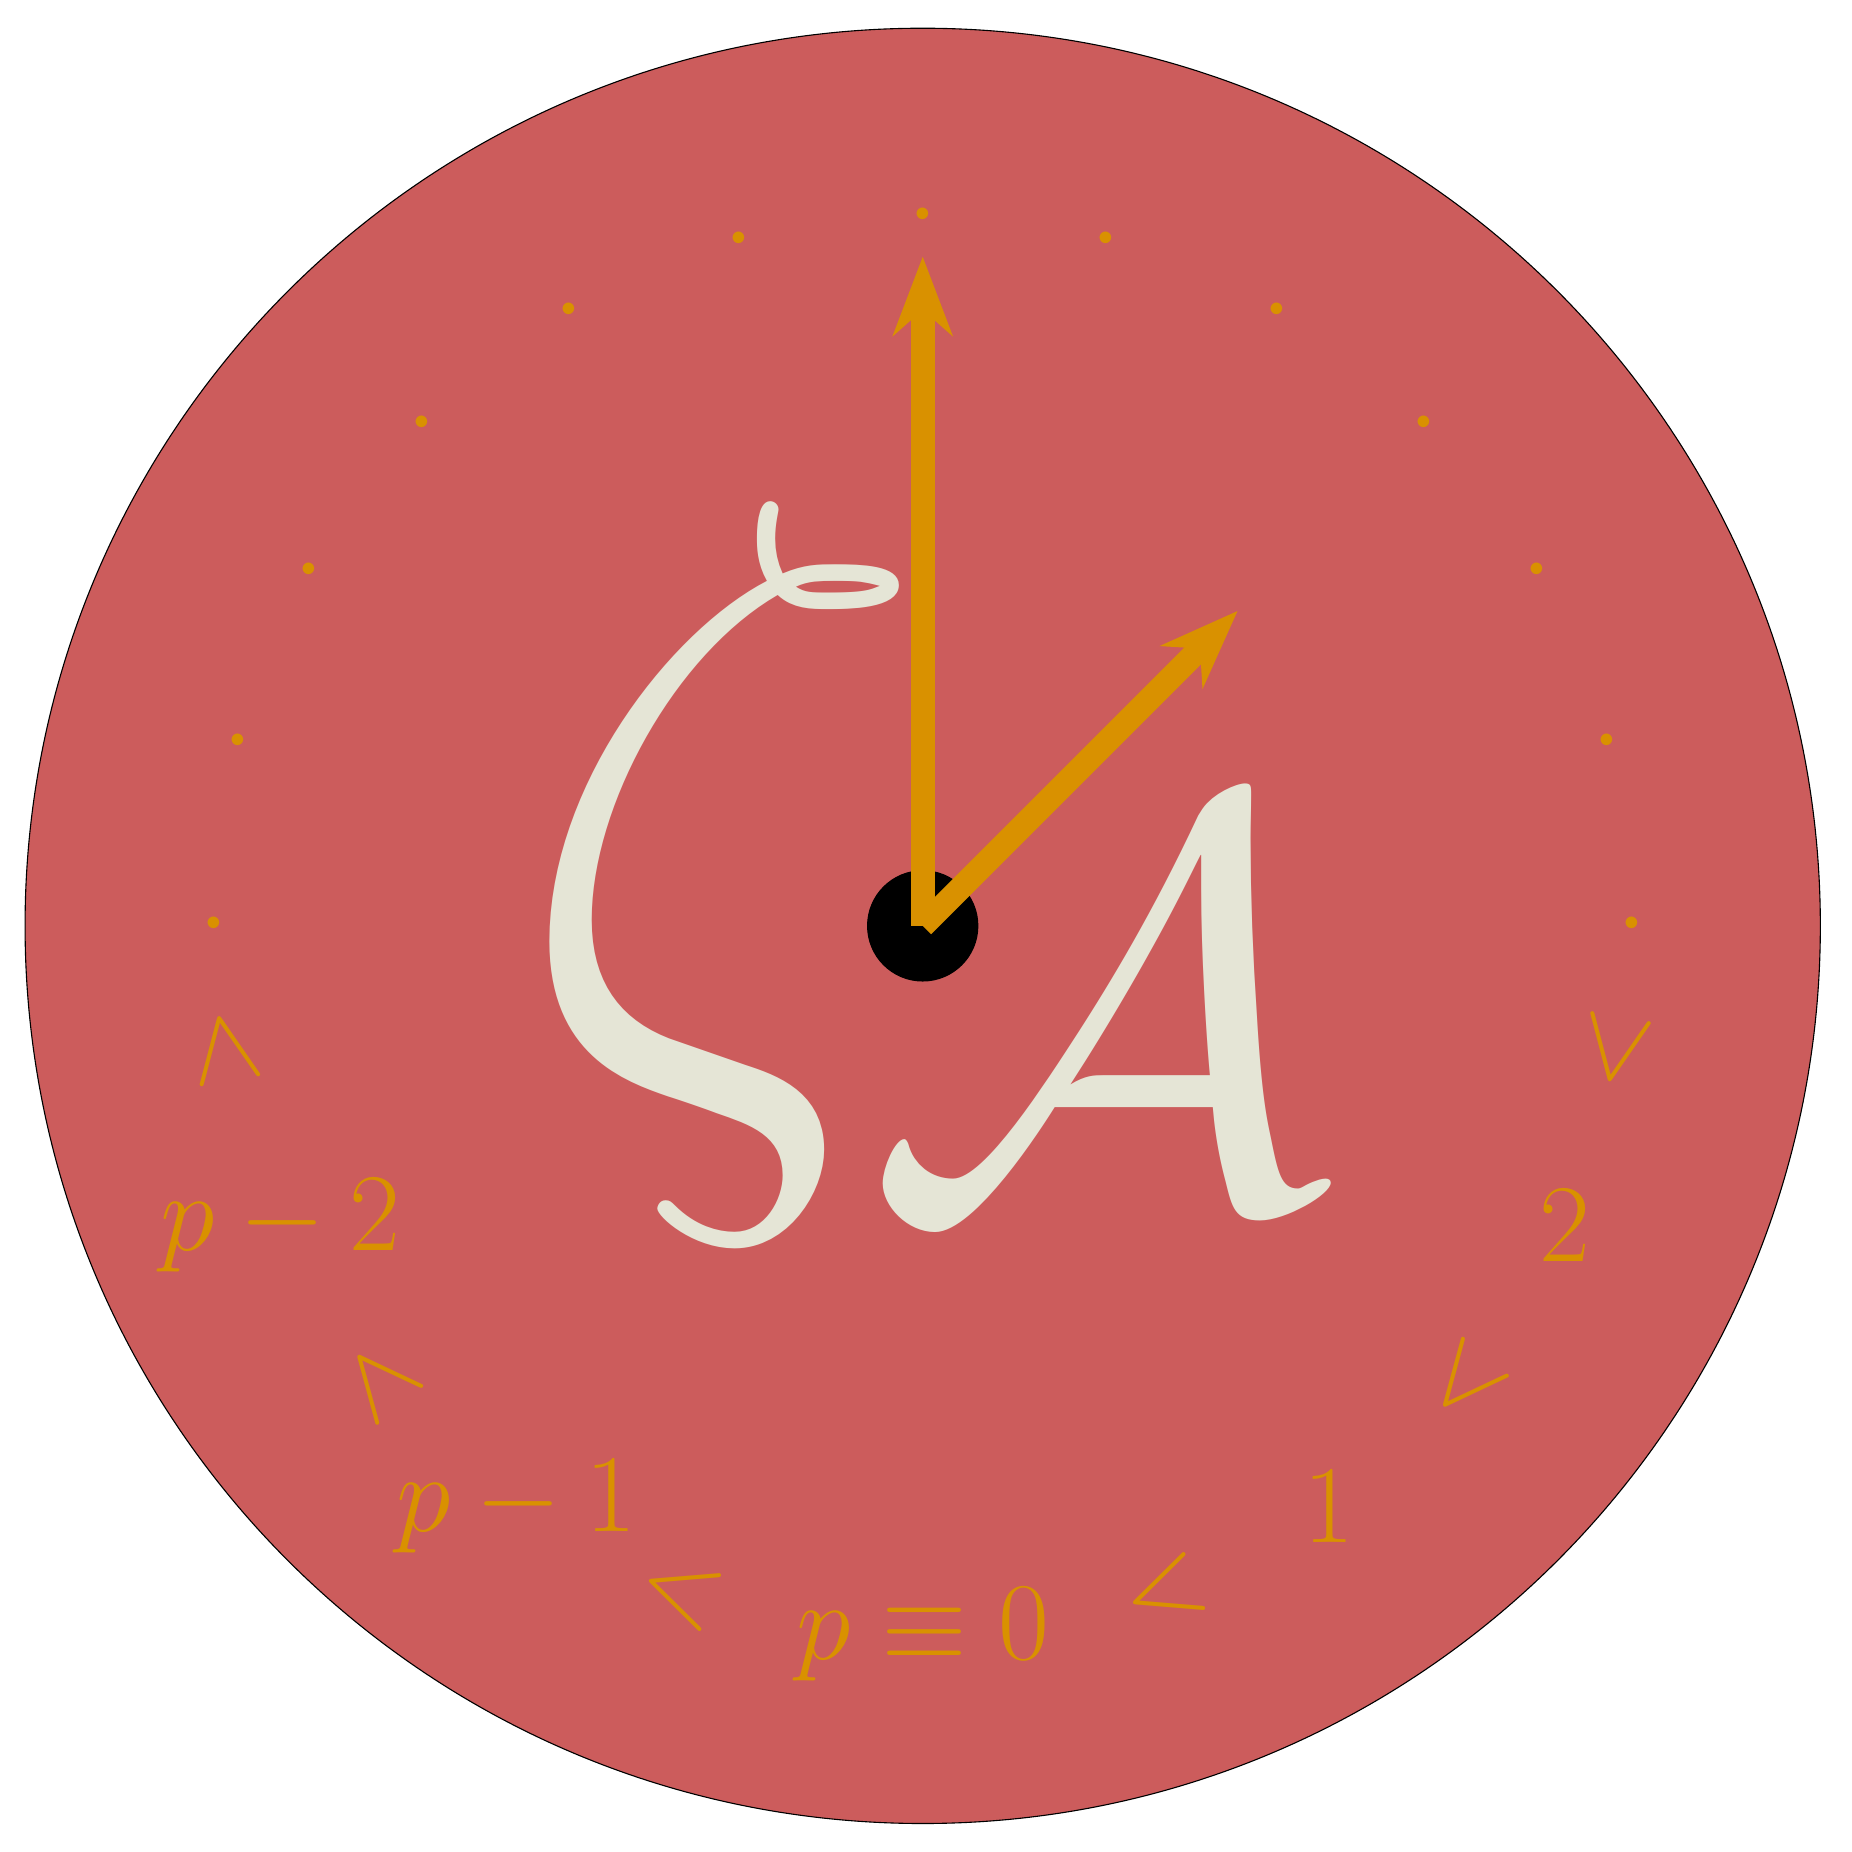
\begin{tikzpicture}
      \coordinate (O) at (0,0);
      \coordinate (OO) at (0,5.5);
      \coordinate (A) at (0,-2);
      \coordinate (B) at (1.29377,-0.759051);
      \coordinate (C) at (1.53209,-1.28558);
    
      \draw [fill=indianred](O) circle (11.4cm);
      \draw [fill=black] (O) circle (7mm);
      % \draw (0,-2) node [anchor=north]{\fontsize{20}{10}{\textit{\textcolor{red!60!black}{Mathematics with \TeX}}}};
      \draw (OO) node [anchor=north]{\fontsize{20}{10}{\textit{\textcolor{ivory}{{\fontsize{300pt}{300pt}\selectfont $\displaystyle \zeta_\mathcal{A}$}}}}};
      \draw [harvestgold,line width=3mm, -{Stealth[length=10mm, open]}] (O) -- (0,8.5);
      \draw [harvestgold,line width=3mm, -{Stealth[length=10mm, open]}] (O) -- (4,4);
      \foreach \angle / \label in 
      {
        % 0/\fontsize{50}{10}{\textcolor{harvestgold}{\rotatebox{90}{$\prec$}}},
        % 30/\fontsize{50}{10}{\textcolor{harvestgold}{\rotatebox{120}{$\cdots$}}},
        % % 60/\fontsize{50}{10}{\textcolor{harvestgold}{$f$}},
        % 90/\fontsize{50}{10}{\textcolor{harvestgold}{$(-\infty=\infty)$}},
        % % 120/\fontsize{50}{10}{\textcolor{harvestgold}{$f$}},
        % 150/\fontsize{50}{10}{\textcolor{harvestgold}{$f$}},
        % 180/\fontsize{50}{10}{\textcolor{harvestgold}{\rotatebox{90}{$\prec$}}},
        % 210/\fontsize{50}{10}{\textcolor{harvestgold}{$\displaystyle -1$}},
        % 240/\fontsize{50}{10}{\textcolor{harvestgold}{\rotatebox{-30}{$\prec$}}},
        % 270/\fontsize{50}{10}{\textcolor{harvestgold}{$\displaystyle (0)$}},
        % 300/\fontsize{50}{10}{\textcolor{harvestgold}{\rotatebox{30}{$\prec$}}},
        % 330/\fontsize{50}{10}{\textcolor{harvestgold}{$\displaystyle 1$}}
        % 
        % 0/$\cdot$, 15/$\cdot$, 30/$\cdot$, 45/$\cdot$, 60/$\cdot$,75/$\cdot$, 90/$\cdot$, 
        % 105/$\cdot$, 120/$\cdot$, 135/$\cdot$, 150/$\cdot$, 165/$\cdot$,
        % 180/$\cdot$, 190/\rotatebox{100}{$>$}, 205/$p-2\ $, 220/\rotatebox{130}{$>$}, 235/$p-1\ $, 
        % 250/\rotatebox{160}{$>$}, 270/$p\equiv 0$, 290/\rotatebox{200}{$>$}, 305/$\ \ 1$, 
        % 320/\rotatebox{230}{$>$}, 335/$\ \ 2$, 350/\rotatebox{260}{$>$}
        % 
        0/\fontsize{40}{10}{\textcolor{harvestgold}{$\cdot$}}, 
        15/\fontsize{40}{10}{\textcolor{harvestgold}{$\cdot$}}, 
        30/\fontsize{40}{10}{\textcolor{harvestgold}{$\cdot$}}, 
        45/\fontsize{40}{10}{\textcolor{harvestgold}{$\cdot$}}, 
        60/\fontsize{40}{10}{\textcolor{harvestgold}{$\cdot$}}, 
        75/\fontsize{40}{10}{\textcolor{harvestgold}{$\cdot$}}, 
        90/\fontsize{40}{10}{\textcolor{harvestgold}{$\cdot$}}, 
        105/\fontsize{40}{10}{\textcolor{harvestgold}{$\cdot$}}, 
        120/\fontsize{40}{10}{\textcolor{harvestgold}{$\cdot$}},
        135/\fontsize{40}{10}{\textcolor{harvestgold}{$\cdot$}}, 
        150/\fontsize{40}{10}{\textcolor{harvestgold}{$\cdot$}}, 
        165/\fontsize{40}{10}{\textcolor{harvestgold}{$\cdot$}},
        180/\fontsize{40}{10}{\textcolor{harvestgold}{$\cdot$}}, 
        190/\fontsize{40}{10}{\textcolor{harvestgold}{\rotatebox{-80}{$<$}}}, 
        205/\fontsize{40}{10}{\textcolor{harvestgold}{$p-2$}}, 
        220/\fontsize{40}{10}{\textcolor{harvestgold}{\rotatebox{-50}{$<$}}}, 
        235/\fontsize{40}{10}{\textcolor{harvestgold}{$p-1$}}, 
        250/\fontsize{40}{10}{\textcolor{harvestgold}{\rotatebox{-20}{$<$}}}, 
        270/\fontsize{40}{10}{\textcolor{harvestgold}{$p\equiv 0$}}, 
        290/\fontsize{40}{10}{\textcolor{harvestgold}{\rotatebox{20}{$<$}}}, 
        305/\fontsize{40}{10}{\textcolor{harvestgold}{$1$}}, 
        320/\fontsize{40}{10}{\textcolor{harvestgold}{\rotatebox{50}{$<$}}}, 
        335/\fontsize{40}{10}{\textcolor{harvestgold}{$2$}}, 
        350/\fontsize{40}{10}{\textcolor{harvestgold}{\rotatebox{80}{$<$}}
        }
      } 
      { 
      %  \draw (\angle:22cm) -- (\angle:12cm); 
       \node at (\angle:9cm) {\textsf{\label}}; 
      } 
    \end{tikzpicture}
    
    \newpage
    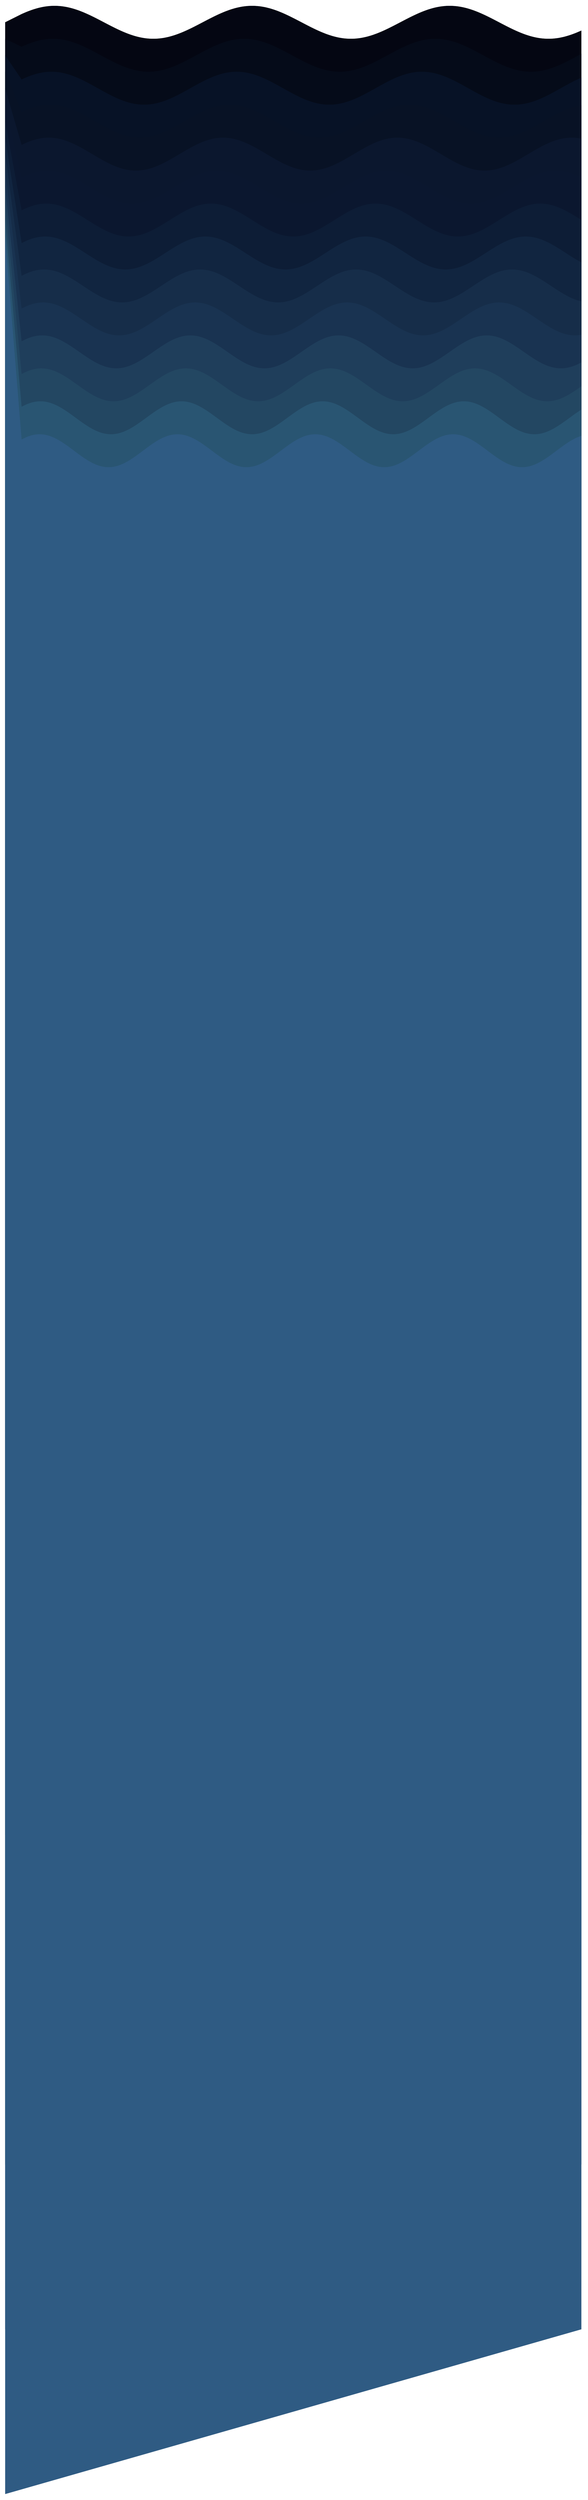
\begin{tikzpicture}
      \coordinate (O) at (0,0);
      \coordinate (A) at (1,0);
      \coordinate (B) at (0,1);

      % \fill [fill=black1] (A) to [out=0,in=90] (B);
      % \fill [fill=black2] (O) circle (13cm);
      % \fill [fill=black3] (O) circle (12cm);
      % \fill [fill=black4] (O) circle (11cm);
      % \fill [fill=black5] (O) circle (10cm);
      % \fill [fill=black6] (O) circle (9cm);
      % \fill [fill=black7] (O) circle (8cm);
      % \fill [fill=black8] (O) circle (7cm);
      % \fill [fill=black9] (O) circle (6cm);
      % \fill [fill=black10] (O) circle (5cm);
      % \fill [fill=black11] (O) circle (4cm);
      % \fill [fill=black12] (O) circle (3cm);
      % \fill [fill=black13] (O) circle (2cm);
      % \fill [fill=black14] (O) circle (1cm);
      \fill [fill=blue1] [smooth,samples=100,domain=35:1] plot (\x,{sin(30*\x)}) --(0,0) --(0,-20) -- (35,-20);
      \fill [fill=blue2] [smooth,samples=100,domain=35:1] plot (\x,{sin(31*\x)-2}) --(0,-1) --(0,-30) -- (35,-30);
      \fill [fill=blue3] [smooth,samples=100,domain=35:1] plot (\x,{sin(32*\x)-4}) --(0,-2) --(0,-40) -- (35,-40);
      \fill [fill=blue4] [smooth,samples=100,domain=35:1] plot (\x,{sin(33*\x)-6}) --(0,-3) --(0,-50) -- (35,-50);
      \fill [fill=blue5] [smooth,samples=100,domain=35:1] plot (\x,{sin(34*\x)-8}) --(0,-4) --(0,-60) -- (35,-60);
      \fill [fill=blue6] [smooth,samples=100,domain=35:1] plot (\x,{sin(35*\x)-10}) --(0,-5) --(0,-70) -- (35,-70);
      \fill [fill=blue7] [smooth,samples=100,domain=35:1] plot (\x,{sin(36*\x)-12}) --(0,-6) --(0,-80) -- (35,-80);
      \fill [fill=blue8] [smooth,samples=100,domain=35:1] plot (\x,{sin(37*\x)-14}) --(0,-7) --(0,-90) -- (35,-90);
      \fill [fill=blue9] [smooth,samples=100,domain=35:1] plot (\x,{sin(38*\x)-16}) --(0,-8) --(0,-100) -- (35,-90);
      \fill [fill=blue10] [smooth,samples=100,domain=35:1] plot (\x,{sin(39*\x)-18}) --(0,-9) --(0,-110) -- (35,-100);
      \fill [fill=blue11] [smooth,samples=100,domain=35:1] plot (\x,{sin(40*\x)-20}) --(0,-10) --(0,-120) -- (35,-110);
      \fill [fill=blue12] [smooth,samples=100,domain=35:1] plot (\x,{sin(41*\x)-22}) --(0,-11) --(0,-130) -- (35,-120);
      \fill [fill=blue13] [smooth,samples=100,domain=35:1] plot (\x,{sin(42*\x)-24}) --(0,-12) --(0,-140) -- (35,-130);
      \fill [fill=blue14] [smooth,samples=100,domain=35:1] plot (\x,{sin(43*\x)-26}) --(0,-13) --(0,-150) -- (35,-140);
      % \draw [smooth,samples=100,domain=0.035:1] plot(\x,{\x - ln(\x) - 1});
    \end{tikzpicture}
\end{document}